\documentclass[lang=cn,newtx,10pt,scheme=chinese]{elegantbook}

\title{深入浅出数据结构}
\subtitle{北街学长倾力之作}

\author{北街}
% \institute{Elegant\LaTeX{} Program}
\date{2022/12/31}
\version{1.0}
% \bioinfo{自定义}{信息}

% \extrainfo{注意:本模板自 2023 年 1 月 122222 日开始,不再更新和维护!}

\setcounter{tocdepth}{3}

\logo{logo-blue.png}
\cover{cover.jpg}

% 本文档命令
\usepackage{array}
\newcommand{\ccr}[1]{\makecell{{\color{#1}\rule{1cm}{1cm}}}}

% 修改标题页的橙色带
\definecolor{customcolor}{RGB}{32,178,170}
\colorlet{coverlinecolor}{customcolor}
\usepackage{cprotect}

\addbibresource[location=local]{reference.bib} % 参考文献,不要删除
\usepackage{listings}         % 导入listings宏包
\usepackage{xcolor}           % 支持颜色

% 配置C++代码样式
\lstset{
    language=C++,             % 语言设置为C++
    basicstyle=\ttfamily,      % 基本样式
    keywordstyle=\color{blue}, % 关键词颜色
    commentstyle=\color{green},% 注释颜色
    stringstyle=\color{red},   % 字符串颜色
    numbers=left,              % 显示行号
    numberstyle=\tiny,         % 行号样式
    stepnumber=1,              % 每行显示行号
    breaklines=true,           % 自动换行
    frame=lines                % 代码块边框样式
}
\begin{document}

\maketitle
\frontmatter

\tableofcontents

\mainmatter

\chapter{数据结构与算法}

\section{数据结构}

\subsection{定义}
数据结构是什么?简单来说,它是用来组织和存储数据的一种方式。就像你整理房间时,衣服放衣柜,书籍放书架,零食藏在抽屉里(别骗我,你一定有零食抽屉!)。数据结构就是计算机世界里的“收纳神器”,它决定了数据的存储方式和操作效率。

\subsection{逻辑结构}
逻辑结构是数据之间的关系,就像你和朋友之间的关系一样复杂(或者简单)。根据数据元素之间的关系,逻辑结构可以分为以下几类:
\begin{itemize}
    \item \textbf{集合结构}:数据之间没有任何关系,就像一群互不认识的人站在公交车站。
    \item \textbf{线性结构}:数据之间有一对一的关系,就像排队买奶茶,每个人前后都有一个邻居。
    \item \textbf{树形结构}:数据之间有一对多的关系,就像家谱,祖宗有很多子孙。
    \item \textbf{图形结构}:数据之间有多对多的关系,就像社交网络,人人都可能是朋友(或者敌人)。
\end{itemize}

\subsection{存储结构}
存储结构是数据在计算机中的存储方式,决定了数据的“住址”。主要有以下两种:
\begin{itemize}
    \item \textbf{顺序存储}:数据存储在连续的存储单元中,就像一排整齐的书架。优点是访问速度快,缺点是插入和删除操作麻烦。
    \item \textbf{链式存储}:数据存储在不连续的存储单元中,通过指针连接,就像一串珍珠项链。优点是插入和删除方便,缺点是访问速度稍慢。
\end{itemize}
选择哪种存储方式,就像选择住公寓还是住别墅,各有利弊,关键看需求。

\section{算法}

\subsection{定义}
算法是解决问题的一组明确指令。它就像做菜的菜谱,告诉你每一步该干什么。比如,“煮方便面”这个算法可能是这样的:
\begin{enumerate}
    \item 烧水。
    \item 水开后放入面饼。
    \item 等3分钟,加入调料包。
    \item 搅拌均匀,开吃!
\end{enumerate}
一个好的算法不仅要能解决问题,还要高效,毕竟没人想等水烧开等到天荒地老。

\subsection{特征}
算法有以下几个显著特征:
\begin{itemize}
    \item \textbf{有穷性}:算法必须在有限步骤内结束,就像煮方便面不能煮一辈子。
    \item \textbf{确定性}:算法的每一步都有明确的定义,不会让你“随便加点盐”。
    \item \textbf{可行性}:算法的每一步都可以通过基本操作实现,比如“烧水”是可行的,但“召唤龙卷风”就不行。
    \item \textbf{输入}:算法可以有零个或多个输入,比如煮方便面需要水和面饼。
    \item \textbf{输出}:算法至少有一个输出,比如煮好的方便面。
\end{itemize}

\subsection{目标}
设计算法的目标是让它又快又省。具体来说:
\begin{itemize}
    \item \textbf{减少时间复杂度}:让算法运行得更快,就像希望快递能当天送达。
    \item \textbf{减少空间复杂度}:让算法占用更少的内存,就像希望行李箱能装下更多东西。
\end{itemize}
一个好的算法就像一个优秀的厨师,既能快速做好饭,又不浪费食材。

\subsection{复杂度计算}
算法复杂度是衡量算法效率的重要指标,分为时间复杂度和空间复杂度。它们是评估算法性能的核心标准,就像评估一辆车的油耗和速度,既要省油又要跑得快才是好车。

\subsubsection{时间复杂度}
时间复杂度描述算法运行所需的时间,通常用大 $O$ 表示法来表示。以下是一些常见的时间复杂度及其含义:

\begin{itemize}
    \item \textbf{$O(1)$:常数时间}
    无论输入规模多大,算法的运行时间都保持不变。
    \textit{示例}:访问数组中的某个元素,例如 $arr[5]$。
    \textit{解释}:直接定位到数组的第六个元素(索引从 0 开始),不需要额外的计算。

    \item \textbf{$O(n)$:线性时间}
    算法的运行时间与输入规模成正比。
    \textit{示例}:计算一个数组中所有元素的和。
    \textit{解释}:假设数组有 $n$ 个元素,算法需要遍历每个元素一次,因此运行时间为 $O(n)$。

    \item \textbf{$O(n^2)$:平方时间}
    算法的运行时间与输入规模的平方成正比。
    \textit{示例}:对一个数组中的所有元素两两比较,例如冒泡排序。
    \textit{解释}:对于 $n$ 个元素,每个元素需要与其他 $n-1$ 个元素进行比较,总共需要执行 $n \times (n-1)$ 次操作,近似为 $O(n^2)$。

    \item \textbf{$O(\log n)$:对数时间}
    算法的运行时间随着输入规模的对数增长。
    \textit{示例}:在一个有序数组中使用二分查找。
    \textit{解释}:每次查找都会将搜索范围缩小一半,因此运行时间为 $O(\log n)$。

    \item \textbf{$O(n \log n)$:线性对数时间}
    常见于高效的排序算法,例如归并排序和快速排序。
    \textit{示例}:对一个数组进行快速排序。
    \textit{解释}:快速排序在每次划分时需要 $O(n)$ 的时间,而划分的次数为 $O(\log n)$,因此总时间复杂度为 $O(n \log n)$。
\end{itemize}

\textbf{计算示例:}
假设我们有一个数组 $arr = [3, 1, 4, 1, 5]$,我们想要计算数组中所有元素的平方和:
\begin{verbatim}
for i in arr:
    result += i * i
\end{verbatim}
该算法需要遍历数组中的每个元素一次,因此时间复杂度为 $O(n)$。

\subsubsection{空间复杂度}
空间复杂度描述算法运行所需的存储空间,通常也用大 $O$ 表示法。以下是一些常见的空间复杂度及其含义:

\begin{itemize}
    \item \textbf{$O(1)$:常数空间}
    算法所需的额外空间不随输入规模的变化而变化。
    \textit{示例}:交换两个变量的值。
    \textit{解释}:只需要一个临时变量来存储中间值,额外空间为常数。

    \item \textbf{$O(n)$:线性空间}
    算法所需的额外空间与输入规模成正比。
    \textit{示例}:创建一个与输入数组大小相同的数组来存储结果。
    \textit{解释}:如果输入数组有 $n$ 个元素,额外需要 $n$ 个存储单元。

    \item \textbf{$O(n^2)$:平方空间}
    算法所需的额外空间与输入规模的平方成正比。
    \textit{示例}:创建一个 $n \times n$ 的二维矩阵。
    \textit{解释}:如果矩阵的维度为 $n$,则需要 $n^2$ 个存储单元。
\end{itemize}

\textbf{计算示例:}
假设我们需要存储一个二维数组的转置矩阵:
\begin{verbatim}
for i in range(n):
    for j in range(n):
        transpose[j][i] = matrix[i][j]
\end{verbatim}
如果原始矩阵的大小为 $n \times n$,则需要额外的 $n^2$ 空间来存储转置矩阵,因此空间复杂度为 $O(n^2)$。

\subsubsection{综合示例}
假设我们需要对一个数组进行排序并统计其中每个元素出现的次数:
\begin{itemize}
    \item 排序算法使用快速排序,时间复杂度为 $O(n \log n)$。
    \item 统计元素出现次数需要一个哈希表,空间复杂度为 $O(n)$。
\end{itemize}
因此,该算法的总时间复杂度为 $O(n \log n)$,空间复杂度为 $O(n)$。

通过这些示例,我们可以更直观地理解时间复杂度和空间复杂度的概念。复杂度计算就像评估一辆车的性能,既要跑得快(时间复杂度低),又要省油(空间复杂度低),才能称得上是一辆好车。

\chapter{线性表}

\section{线性表的逻辑结构}
线性表是一种最基本、最常用的数据结构,它的特点是数据元素之间存在一对一的线性关系。可以把它想象成排队买奶茶的队伍,每个人前后都有一个邻居,队伍的顺序非常重要。

线性表的逻辑结构可以用数学形式表示为:
$L = \{a_1, a_2, \dots, a_n\}$,其中 $a_i$ 表示线性表中的第 $i$ 个元素,$1 \leq i \leq n$。
\textit{示例}:假设线性表存储的是一周的日程安排:
$L = \{\text{周一}, \text{周二}, \text{周三}, \text{周四}, \text{周五}\}$。

线性表的特点:
\begin{itemize}
    \item 有且仅有一个“第一个”元素(队伍的开头)。
    \item 有且仅有一个“最后一个”元素(队伍的末尾)。
    \item 除了第一个和最后一个元素外,每个元素都有一个前驱和一个后继。
\end{itemize}

\section{顺序表}

\subsection{顺序表的定义}
顺序表是一种线性表的存储结构,它使用一组地址连续的存储单元依次存储线性表中的数据元素。可以把它想象成一排整齐的书架,每本书都有固定的位置。

\textit{示例}:假设我们有一个顺序表存储学生的学号:
$L = \{1001, 1002, 1003, 1004\}$。
在内存中,它可能被存储为:
\begin{table}[h]
  \centering
  \begin{tabular}{|c|c|c|c|c|}
  \hline
  \textbf{地址} & 0 & 1 & 2 & 3 \\
  \hline
  \textbf{数据} & 1001 & 1002 & 1003 & 1004 \\
  \hline
  \end{tabular}
  \caption{顺序表的存储示例}
  \label{tab:sequence_table}
\end{table}
顺序表的优点:
\begin{itemize}
    \item 支持随机访问,可以通过下标快速访问任意元素,时间复杂度为 $O(1)$。
    \item 存储结构简单,容易实现。
\end{itemize}

顺序表的缺点:
\begin{itemize}
    \item 插入和删除操作效率较低,时间复杂度为 $O(n)$。
    \item 需要连续的存储空间,可能导致内存浪费或溢出。
\end{itemize}

\subsection{顺序表的操作}
顺序表的基本操作包括插入、删除、查找和更新。以下是每种操作的详细说明:

\textbf{创建操作}:
创建一个空的顺序表,需要预先分配一定的存储空间。然后根据实际需求逐个插入元素。
代码如代码\ref{lst:create_list}所示:
\begin{lstlisting}[language=C++, caption={顺序表的创建示例代码}, label={lst:create_list}]
  #include <stdio.h>
  #include <stdlib.h>
  #define MAXSIZE 100

  typedef struct {//C语言方式
    int data[MAXSIZE];
    int length;
  }SqList;

  struct SqList {//c++方式,个人推荐这种方式,简单
    int data[MAXSIZE];
    int length;
  };
  SqList* createList(int length) {//传入要创建的顺序表的长度
    SqList* L = (SqList*)malloc(sizeof(SqList) * length);//分配存放线性表的空间
    int data;
    for (int i = 0; i < length; i++)
    {
      printf("请输入第%d个元素", i);
      scanf("%d", &L->data[i]);
    }
    L->length = length;
    return L;
  }
  \end{lstlisting}

时间复杂度为$O(n)$。很明显,这个操作用到了单层循环,所以时间复杂度为$O(n)$,

空间复杂度为$O(n)$。这里用到了一个数组,数组的长度为n,所以空间复杂度为$O(n)$。

\textbf{插入操作}:
在顺序表的第 $i$ 个位置插入一个新元素,需要将第 $i$ 个位置及其后的所有元素向后移动一位。
\textit{示例}:在 $L = \{1001, 1002, 1003, 1004\}$ 的第 2 个位置插入 $1005$,结果为:
$L = \{1001, 1005, 1002, 1003, 1004\}$。代码如代码\ref{lst:insert_list}所示:
\begin{lstlisting}[language=C++, caption={顺序表的插入示例代码}, label={lst:insert_list}]
  void insertList(SqList* L, int i, int data) {//传入要插入的顺序表,要插入的位置,要插入的数据
    if (i < 0 || i > L->length) {
      printf("插入位置不合法");
      return;
    }
    for (int j = L->length; j > i; j--)
    {
      L->data[j] = L->data[j - 1];
    }
    L->data[i] = data;
    L->length++;
  }
  \end{lstlisting}
时间复杂度为$O(n)$。很明显,这个操作用到了单层循环,所以时间复杂度为$O(n)$,
空间复杂度为$O(1)$。这里只用到了几个变量,所以空间复杂度为$O(1)$。



\textbf{删除操作}:
删除顺序表的第 $i$ 个元素,需要将第 $i+1$ 个位置及其后的所有元素向前移动一位。
\textit{示例}:从 $L = \{1001, 1002, 1003, 1004\}$ 中删除第 3 个元素,结果为:
$L = \{1001, 1002, 1004\}$。代码如代码\ref{lst:delete_list}所示:
\begin{lstlisting}[language=C++, caption={顺序表的删除示例代码}, label={lst:delete_list}]
  void deleteList(SqList* L, int i) {//传入要删除的顺序表,要删除的位置
    if (i < 0 || i >= L->length) {
      printf("删除位置不合法");
      return;
    }
    for (int j = i; j < L->length - 1; j++)
    {
      L->data[j] = L->data[j + 1];
    }
    L->length--;
  }
  \end{lstlisting}
时间复杂度为$O(n)$。很明显,这个操作用到了单层循环,所以时间复杂度为$O(n)$,
空间复杂度为$O(1)$。这里只用到了几个变量,所以空间复杂度为$O(1)$。

\textbf{查找操作}:
根据元素的值查找其在顺序表中的位置,时间复杂度为 $O(n)$。
\textit{示例}:在 $L = \{1001, 1002, 1003, 1004\}$ 中查找 $1003$,结果为位置 3。
代码如代码\ref{lst:search_list}所示:
\begin{lstlisting}[language=C++, caption={顺序表的查找示例代码}, label={lst:search_list}]
  int searchList(SqList* L, int data) {//传入要查找的顺序表,要查找的数据
    for (int i = 0; i < L->length; i++)
    {
      if (L->data[i] == data) {
        return i;
      }
    }
    return -1;
  }
  \end{lstlisting}
时间复杂度为$O(n)$。很明显,这个操作用到了单层循环,所以时间复杂度为$O(n)$,
空间复杂度为$O(1)$。这里只用到了几个变量,所以空间复杂度为$O(1)$。

\textbf{更新操作}:
将顺序表中第 $i$ 个位置的元素更新为新的值。
\textit{示例}:将 $L = \{1001, 1002, 1003, 1004\}$ 中第 2 个元素更新为 $2002$,结果为:
$L = \{1001, 2002, 1003, 1004\}$。
代码如代码\ref{lst:update_list}所示:
\begin{lstlisting}[language=C++, caption={顺序表的更新示例代码}, label={lst:update_list}]
  void updateList(SqList* L, int i, int data) {//传入要更新的顺序表,要更新的位置,要更新的数据
    if (i < 0 || i >= L->length) {
      printf("更新位置不合法");
      return;
    }
    L->data[i] = data;
  }
  \end{lstlisting}
时间复杂度为$O(1)$。很明显,这个操作只用到了一次赋值操作,所以时间复杂度为$O(1)$,
空间复杂度为$O(1)$。这里只用到了几个变量,所以空间复杂度为$O(1)$。

\section{链表}

\subsection{链表的定义}
链表是一种线性表的存储结构,它使用一组任意的存储单元存储数据元素,并通过指针将这些存储单元连接起来。可以把它想象成一串珍珠项链,每颗珍珠(数据元素)通过线(指针)连接在一起。

链表的优点:
\begin{itemize}
    \item 插入和删除操作效率高,时间复杂度为 $O(1)$。
    \item 不需要连续的存储空间,内存利用率高。
\end{itemize}

链表的缺点:
\begin{itemize}
    \item 不支持随机访问,查找效率较低,时间复杂度为 $O(n)$。
    \item 需要额外的存储空间存储指针。
\end{itemize}

\subsection{链表的相关术语}
\begin{itemize}
  \item \textbf{头指针}:指向链表的第一个节点的指针。
  \item \textbf{尾指针}:指向链表的最后一个节点的指针。
  \item \textbf{头结点}:不存储数据的节点,用于标识链表的起始位置。
  \item \textbf{尾结点}:指向 NULL 的节点,表示链表的结束。
  \item \textbf{首元结点}:第一个存储数据的节点。
\end{itemize}
为什么链表需要头结点?头结点是链表的起始位置,它不存储数据,只是为了方便操作。有了头结点,我们可以通过头指针快速访问链表的第一个节点,而无需特殊处理。
常见的单链表如图\ref{fig:single_linked_list}所示,常见的双链表如图\ref{fig:double_linked_list}所示。
\begin{figure}[h]
  \centering
  \includegraphics[width=0.8\textwidth]{./image/singleLink.png}
  \caption{单链表表示意图}
  \label{fig:single_linked_list}
\end{figure}

\begin{figure}[h]
  \centering
  \includegraphics[width=0.8\textwidth]{./image/doubleLink.png}
  \caption{双链表示意图}
  \label{fig:double_linked_list}
\end{figure}

\subsubsection{单链表}
单链表是链表的一种,每个节点只包含一个数据域和一个指针域,指针指向下一个节点。
\textit{示例}:
$L = \{1001 \rightarrow 1002 \rightarrow 1003\}$。
单链表的结构如图\ref{fig:singleLinkStruct}所示。单链表的结构由数据域和指针域组成,其中数据域存储数据元素,指针域存储下一个节点的地址。
\begin{figure}[h]
  \centering
  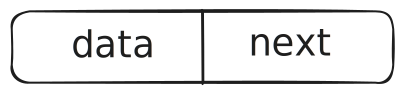
\includegraphics[width=0.6\textwidth]{./figure/pdf/cropped/singleStruct.pdf}
  \caption{单链表结构}
  \label{fig:singleLinkStruct}
\end{figure}
单链表的结构体定义如代码\ref{lst:singleLinkStruct}所示。
\begin{lstlisting}[language=C++, caption={单链表结构体定义}, label={lst:singleLinkStruct}]
  struct ListNode {
    int data;
    ListNode* next;
  };
\end{lstlisting}
单链表的基本操作包括插入、删除、查找和更新。以下是每种操作的详细说明:
建立单链表:

  头插法建立单链表

  1.首先创建一个头结点,将头结点的指针域指向 NULL。
  2.依次读入数据元素,创建新节点,将新节点的指针域指向头结点的下一个节点,再将头结点的指针域指向新节点。
  具体过程如图\ref{fig:headInsert}所示。
  \begin{figure}[h]
    \centering
    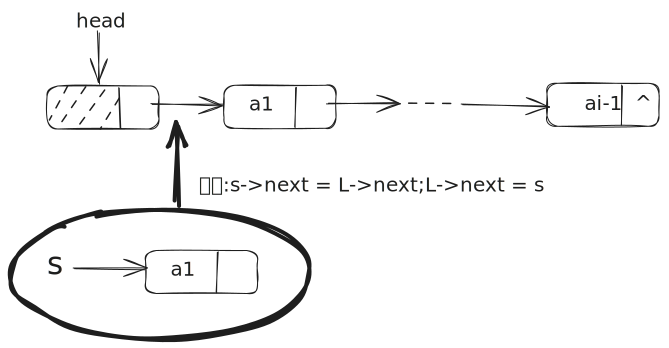
\includegraphics[width=1\textwidth]{./figure/pdf/cropped/headInsert.pdf}
    \caption{头插法建立单链表}
    \label{fig:headInsert}
  \end{figure}
  代码如代码\ref{lst:headInsert}所示。
  \begin{lstlisting}[language=C++, caption={头插法建立单链表示例代码}, label={lst:headInsert}]
    singleLink* createSingleLink() {
      int n, data;
      printf("请输入创建链表的节点个数:");
      scanf("%d", &n);
      SingleLink* L = (SingleLink*)malloc(sizeof(SingleLink));
      L->next = NULL;
      for (int i = 0; i < n; i++) {
        SingleLink* s = (singleLink*)malloc(sizeof(SingleLink));
        printf("请输入第%d个节点的值(int):", i + 1);
        scanf("%d", &data);
        s->data = data;
        s->next = NULL;
        s->next = L->next;
        L->next = s;
      }
      return L;
    }
    \end{lstlisting}
    该算法的总时间复杂度为 $O(n)$,空间复杂度为 $O(1)$。

    特点:头插法建立的单链表,新节点插入到链表的头部,逆序存储数据。

  尾插法建立单链表

  1.首先创建一个头结点,将头结点的指针域指向 NULL。
  2.依次读入数据元素,创建新节点,将新节点的指针域指向 NULL,再将尾结点的指针域指向新节点,再将新节点作为尾结点。
  具体过程如图\ref{fig:tailInsert}所示。
  \begin{figure}[h]
    \centering
    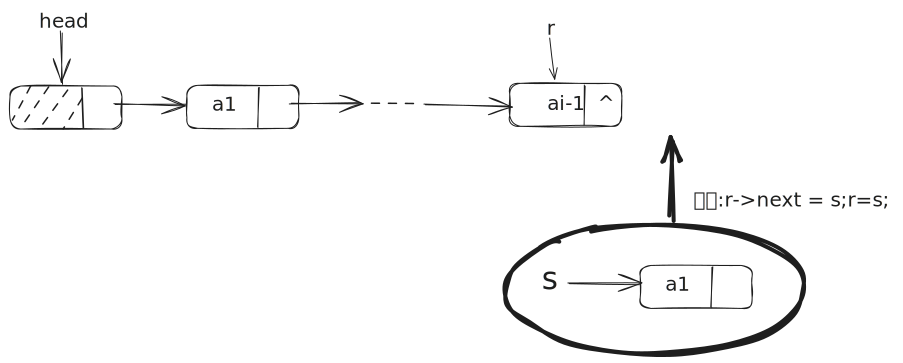
\includegraphics[width=1\textwidth]{./figure/pdf/cropped/tailInsert.pdf}
    \caption{尾插法建立单链表}
    \label{fig:tailInsert}
  \end{figure}
  代码如代码\ref{lst:tailInsert}所示。
  \begin{lstlisting}[language=C++, caption={尾插法建立单链表示例代码}, label={lst:tailInsert}]
    singleLink* createSingleLink() {
      int n, data;
      printf("请输入创建链表的节点个数:");
      scanf("%d", &n);
      SingleLink* L = (SingleLink*)malloc(sizeof(SingleLink));
      SingleLink* r = L;
      for (int i = 0; i < n; i++) {
        SingleLink* s = (singleLink*)malloc(sizeof(SingleLink));
        printf("请输入第%d个节点的值(int):", i + 1);
        scanf("%d", &data);
        s->data = data;
        s->next = NULL;
        r->next = s;
        r = s;
      }
      return L;
    }
    \end{lstlisting}
    该算法的总时间复杂度为 $O(n)$,空间复杂度为 $O(1)$。

    特点:尾插法建立的单链表,新节点插入到链表的尾部,顺序存储数据。

创建一个空链表

创建一个空链表,只需要创建一个头结点,将头结点的指针域指向 NULL。

代码如代码\ref{lst:createEmptySingleLink}所示。
\begin{lstlisting}[language=C++, caption={创建一个空链表示例代码}, label={lst:createEmptySingleLink}]
  singleLink* createEmptySingleLink() {
    SingleLink* L = (SingleLink*)malloc(sizeof(SingleLink));
    L->next = NULL;
    return L;
  }
\end{lstlisting}
该算法的总时间复杂度为 $O(1)$,空间复杂度为 $O(1)$。

特点:创建的链表为空,不包含任何数据元素。

输出单链表

输出单链表的所有数据元素,需要遍历链表的所有节点,并依次输出节点的数据域。

代码如代码\ref{lst:printSingleLink}所示。

\begin{lstlisting}[language=C++, caption={输出单链表示例代码}, label={lst:printSingleLink}]
void printSingleLink(SingleLink* L) {
  SingleLink* p = L->next;
  while (p != NULL) {
    printf("%d ", p->data);
    p = p->next;
  }
  printf("\n");
}
\end{lstlisting}
该算法的总时间复杂度为 $O(n)$,空间复杂度为 $O(1)$。

特点:输出单链表的所有数据元素。

输出单链表的长度

输出单链表的长度,需要遍历链表的所有节点,并统计节点的个数。

代码如代码\ref{lst:lengthSingleLink}所示。

\begin{lstlisting}[language=C++, caption={输出单链表长度示例代码}, label={lst:lengthSingleLink}]
int lengthSingleLink(SingleLink* L) {
  SingleLink* p = L->next;
  int length = 0;
  while (p != NULL) {
    length++;
    p = p->next;
  }
  return length;
}
\end{lstlisting}
该算法的总时间复杂度为 $O(n)$,空间复杂度为 $O(1)$。

特点:输出单链表的长度,即链表中数据元素的个数。

判断单链表是否为空

判断单链表是否为空,只需要判断头结点的指针域是否为 NULL。

代码如代码\ref{lst:isEmptySingleLink}所示。

\begin{lstlisting}[language=C++, caption={判断单链表是否为空示例代码}, label={lst:isEmptySingleLink}]
  bool isEmptySingleLink(SingleLink* L) {
    return L->next == NULL;
  }
  \end{lstlisting}
  该算法的总时间复杂度为 $O(1)$,空间复杂度为 $O(1)$。

  特点:判断单链表是否为空,即链表中是否包含数据元素。

查找单链表的第 $i$ 个元素

查找单链表的第 $i$ 个元素,需要遍历链表的所有节点,直到找到第 $i$ 个节点。

代码如代码\ref{lst:getSingleLink}所示。

\begin{lstlisting}[language=C++, caption={查找单链表的第 $i$ 个元素示例代码}, label={lst:getSingleLink}]
  int getSingleLink(SingleLink* L, int i) {
    SingleLink* p = L->next;
    int j = 1;
    while (p != NULL && j < i) {
      p = p->next;
      j++;
    }
    if (p == NULL || j > i) {
      printf("第%d个元素不存在", i);
      return -1;
    }
    return p->data;
  }
\end{lstlisting}
该算法的总时间复杂度为 $O(n)$,空间复杂度为 $O(1)$。

特点:查找单链表的第 $i$ 个元素,即链表中第 $i$ 个节点的数据元素。

删除单链表的第 $i$ 个元素

删除单链表的第 $i$ 个元素,需要遍历链表的所有节点,直到找到第 $i$ 个节点,然后删除该节点。

代码如代码\ref{lst:deleteSingleLink}所示。

\begin{lstlisting}[language=C++, caption={删除单链表的第 $i$ 个元素示例代码}, label={lst:deleteSingleLink}]
  void deleteSingleLink(SingleLink* L, int i) {
    SingleLink* p = L;
    for (int j = 0; j < i - 1; j++) {
      p = p->next;
    }
    SingleLink* q = p->next;
    p->next = q->next;
    free(q);
  }
  \end{lstlisting}
  该算法的总时间复杂度为 $O(n)$,空间复杂度为 $O(1)$。

  特点:删除单链表的第 $i$ 个元素,即删除链表中第 $i$ 个节点。

插入单链表的第 $i$ 个元素

插入单链表的第 $i$ 个元素,需要遍历链表的所有节点,直到找到第 $i$ 个节点,然后插入新节点。

代码如代码\ref{lst:insertSingleLink}所示。

\begin{lstlisting}[language=C++, caption={插入单链表的第 $i$ 个元素示例代码}, label={lst:insertSingleLink}]
void insertSingleLink(SingleLink* L, int i, int data) {
  SingleLink* p = L;
  for (int j = 0; j < i - 1; j++) {
    p = p->next;
  }
  SingleLink* s = (SingleLink*)malloc(sizeof(SingleLink));
  s->data = data;
  s->next = p->next;
  p->next = s;
}
\end{lstlisting}
该算法的总时间复杂度为 $O(n)$,空间复杂度为 $O(1)$。

特点:插入单链表的第 $i$ 个元素,即在链表中第 $i$ 个节点的位置插入新节点。
   



  \subsubsection{双链表}
  单链表只有指向下一个节点的指针,在某一些应用场合可能并不是那么方便,比如在删除某个节点时,需要找到该节点的前驱节点,而单链表并没有指向前驱节点的指针。双链表就是为了解决这个问题而设计的,它的每个节点有两个指针,一个指向前驱节点,一个指向后继节点。
  
  \textit{示例}:
  $L = \{\text{NULL} \leftrightarrow 1001 \leftrightarrow 1002 \leftrightarrow 1003 \leftrightarrow \text{NULL}\}$。

  双链表的结构如图\ref{fig:doubleLinkStruct}所示。双链表的结构由数据域、前驱指针和后继指针组成,其中数据域存储数据元素,前驱指针指向前一个节点,后继指针指向后一个节点。
  \begin{figure}[h]
    \centering
    
\includegraphics[width=0.6\textwidth]{./figure/pdf/cropped/doubleLinkStruct.pdf}
    \caption{双链表结构}
    \label{fig:doubleLinkStruct}
  \end{figure}

  双链表的结构体定义如代码\ref{lst:doubleLinkStruct}所示。
  \begin{lstlisting}[language=C++, caption={双链表结构体定义}, label={lst:doubleLinkStruct}]
    struct DLink {
      int data;
      DLink* pre;
      DLink* next;
    };
  \end{lstlisting}

  双链表的基本操作包括插入、删除、查找和更新。以下是每种操作的详细说明:

  \textbf{创建操作}:

  创建一个空的双链表,只需要创建一个头结点,将头结点的前驱指针和后继指针都指向 NULL。

  代码如代码\ref{lst:createEmptyDoubleLink}所示。
  \begin{lstlisting}[language=C++, caption={创建一个空双链表示例代码}, label={lst:createEmptyDoubleLink}]
    DLink* createEmptyDoubleLink() {
      DLink* L = (DLink*)malloc(sizeof(DLink));
      L->pre = NULL;
      L->next = NULL;
      return L;
    }
  \end{lstlisting}
  该算法的总时间复杂度为 $O(1)$,空间复杂度为 $O(1)$。

  特点:创建的双链表为空,不包含任何数据元素。

  \textbf{头插法}:

  头插法建立双链表,新节点插入到链表的头部。

  1.首先创建一个头结点,将头结点的前驱指针和后继指针都指向 NULL。

  2.依次读入数据元素,创建新节点,将新节点的前驱指针指向头结点,将新节点的后继指针指向头结点的后继节点,再将头结点的后继指针指向新节点,最后将新节点作为头结点的后继节点。

  具体过程如图\ref{fig:headInsertDouble}所示。
  \begin{figure}[h]
    \centering
    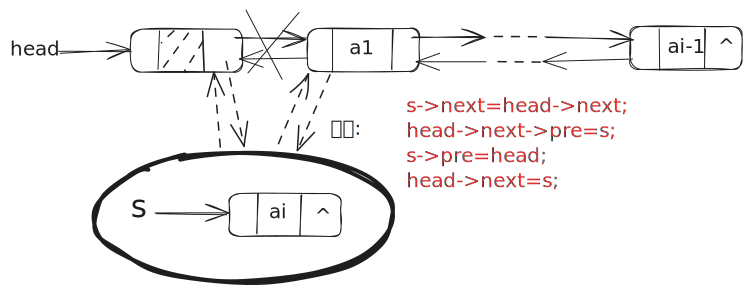
\includegraphics[width=1\textwidth]{./figure/pdf/cropped/headInsertDL.pdf}
    \caption{头插法建立双链表}
    \label{fig:headInsertDouble}
  \end{figure}
  代码如代码\ref{lst:headInsertDouble}所示。
  \begin{lstlisting}[language=C++, caption={头插法建立双链表示例代码}, label={lst:headInsertDouble}]
    DLink* createDoubleLink() {
      int n, data;
      printf("请输入创建链表的节点个数:");
      scanf("%d", &n);
      DLink* L = (DLink*)malloc(sizeof(DLink));
      L->pre = NULL;
      L->next = NULL;
      for (int i = 0; i < n; i++) {
        DLink* s = (DLink*)malloc(sizeof(DLink));
        printf("请输入第%d个节点的值(int):", i + 1);
        scanf("%d", &data);
        s->data = data;
        s->pre = L;
        s->next = L->next;
        L->next = s;
      }
      return L;
    }
  \end{lstlisting}
  该算法的总时间复杂度为 $O(n)$,空间复杂度为 $O(1)$。
  \textbf{尾插法}:
  尾插法建立双链表,新节点插入到链表的尾部。

  1.首先创建一个头结点,将头结点的前驱指针和后继指针都指向 NULL。

  2.依次读入数据元素,创建新节点,将新节点的前驱指针指向尾结点,将新节点的后继指针指向 NULL,再将尾结点的后继指针指向新节点,最后将新节点作为尾结点。

  具体过程如图\ref{fig:tailInsertDouble}所示。
  \begin{figure}[h]
    \centering
    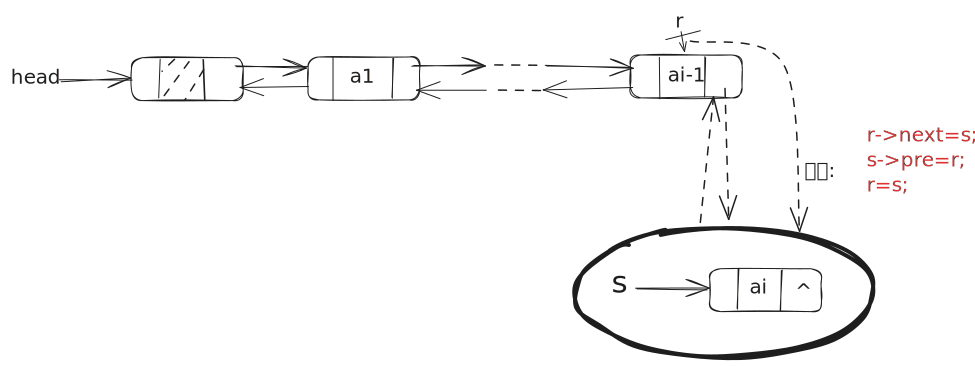
\includegraphics[width=1\textwidth]{./figure/pdf/cropped/tailInsertDL.pdf}
    \caption{尾插法建立双链表}
    \label{fig:tailInsertDouble}
  \end{figure}
  代码如代码\ref{lst:tailInsertDouble}所示。

  \begin{lstlisting}[language=C++, caption={尾插法建立双链表示例代码}, label={lst:tailInsertDouble}]
    DLink* createDoubleLink() {
      int n, data;
      printf("请输入创建链表的节点个数:");
      scanf("%d", &n);
      DLink* L = (DLink*)malloc(sizeof(DLink));
      DLink* r = L;
      for (int i = 0; i < n; i++) {
        DLink* s = (DLink*)malloc(sizeof(DLink));
        printf("请输入第%d个节点的值(int):", i + 1);
        scanf("%d", &data);
        s->data = data;
        s->pre = r;
        s->next = NULL;
        r->next = s;
        r = s;
      }
      return L;
    }
  \end{lstlisting}
  该算法的总时间复杂度为 $O(n)$,空间复杂度为 $O(1)$。

  特点:尾插法建立的双链表,新节点插入到链表的尾部,顺序存储数据。

  \textbf{输出操作}:

  输出双链表的所有数据元素,需要遍历链表的所有节点,并依次输出节点的数据域。

  代码如代码\ref{lst:printDoubleLink}所示。

  \begin{lstlisting}[language=C++, caption={输出双链表示例代码}, label={lst:printDoubleLink}]
    void printDoubleLink(DLink* L) {
      DLink* p = L->next;
      while (p != NULL) {
        printf("%d ", p->data);
        p = p->next;
      }
      printf("\n");
    }
  \end{lstlisting}

  该算法的总时间复杂度为 $O(n)$,空间复杂度为 $O(1)$。

  特点:输出双链表的所有数据元素。

  \textbf{输出双链表的长度}:

  输出双链表的长度,需要遍历链表的所有节点,并统计节点的个数。

  代码如代码\ref{lst:lengthDoubleLink}所示。

  \begin{lstlisting}[language=C++, caption={输出双链表长度示例代码}, label={lst:lengthDoubleLink}]
    int lengthDoubleLink(DLink* L) {
      DLink* p = L->next;
      int length = 0;
      while (p != NULL) {
        length++;
        p = p->next;
      }
      return length;
    }
  \end{lstlisting}

  该算法的总时间复杂度为 $O(n)$,空间复杂度为 $O(1)$。

  特点:输出双链表的长度,即链表中数据元素的个数。

  \textbf{判断双链表是否为空}:

  判断双链表是否为空,只需要判断头结点的后继指针是否为 NULL。

  代码如代码\ref{lst:isEmptyDoubleLink}所示。

  \begin{lstlisting}[language=C++, caption={判断双链表是否为空示例代码}, label={lst:isEmptyDoubleLink}]
    bool isEmptyDoubleLink(DLink* L) {
      return L->next == NULL;
    }
  \end{lstlisting}

  该算法的总时间复杂度为 $O(1)$,空间复杂度为 $O(1)$。

  特点:判断双链表是否为空,即链表中是否包含数据元素。

  \textbf{查找双链表的第 $i$ 个元素}:

  查找双链表的第 $i$ 个元素,需要遍历链表的所有节点,直到找到第 $i$ 个节点。

  代码如代码\ref{lst:getDoubleLink}所示。

  \begin{lstlisting}[language=C++, caption={查找双链表的第 $i$ 个元素示例代码}, label={lst:getDoubleLink}]
    int getDoubleLink(DLink* L, int i) {
      DLink* p = L->next;
      int j = 1;
      while (p != NULL && j < i) {
        p = p->next;
        j++;
      }
      if (p == NULL || j > i) {
        printf("第%d个元素不存在", i);
        return -1;
      }
      return p->data;
    }
  \end{lstlisting}

  该算法的总时间复杂度为 $O(n)$,空间复杂度为 $O(1)$。

  特点:查找双链表的第 $i$ 个元素,即链表中第 $i$ 个节点的数据元素。

  \textbf{删除双链表的第 $i$ 个元素}:

  删除双链表的第 $i$ 个元素,需要遍历链表的所有节点,直到找到第 $i$ 个节点,然后删除该节点。

  代码如代码\ref{lst:deleteDoubleLink}所示。

  \begin{lstlisting}[language=C++, caption={删除双链表的第 $i$ 个元素示例代码}, label={lst:deleteDoubleLink}]
    void deleteDoubleLink(DLink* L, int i) {
      DLink* p = L;
      for (int j = 0; j < i - 1; j++) {
        p = p->next;
      }
      DLink* q = p->next;
      p->next = q->next;
      if (q->next != NULL) {
        q->next->pre = p;
      }
      free(q);
    }
  \end{lstlisting}

  该算法的总时间复杂度为 $O(n)$,空间复杂度为 $O(1)$。

  特点:删除双链表的第 $i$ 个元素,即删除链表中第 $i$ 个节点。

  \textbf{插入双链表的第 $i$ 个元素}:

  插入双链表的第 $i$ 个元素,需要遍历链表的所有节点,直到找到第 $i$ 个节点,然后插入新节点。

  其中删除操作如图\ref{fig:deleteDoubleLink}所示。

  \begin{figure}[h]
    \centering
    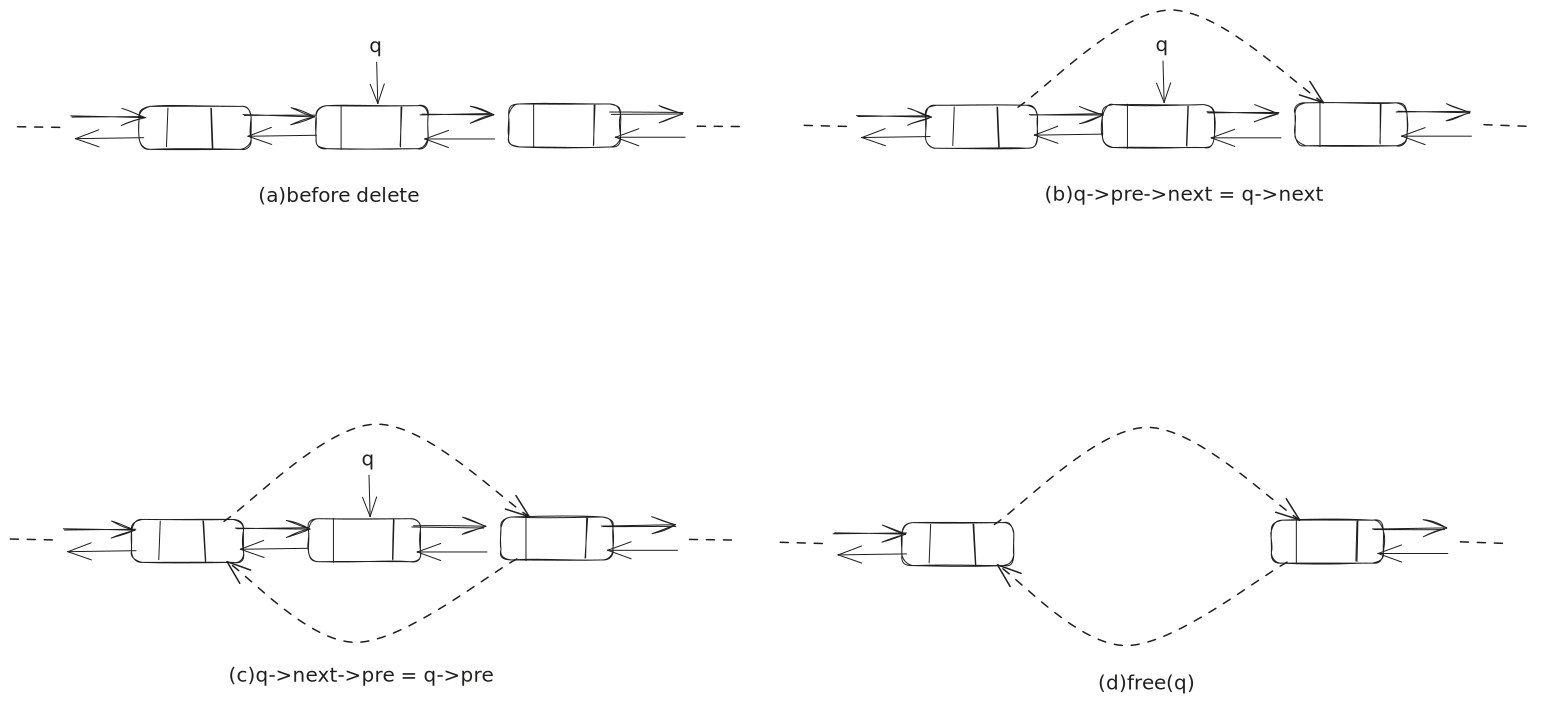
\includegraphics[width=1\textwidth]{./figure/pdf/cropped/deleteDL.pdf}
    \caption{删除双链表的第 $i$ 个元素}
    \label{fig:deleteDoubleLink}
  \end{figure}

  代码如代码\ref{lst:insertDoubleLink}所示。

  \begin{lstlisting}[language=C++, caption={插入双链表的第 $i$ 个元素示例代码}, label={lst:insertDoubleLink}]
    void insertDoubleLink(DLink* L, int i, int data) {
      DLink* p = L;
      for (int j = 0; j < i - 1; j++) {
        p = p->next;
      }
      DLink* s = (DLink*)malloc(sizeof(DLink));
      s->data = data;
      s->pre = p;
      s->next = p->next;
      if (p->next != NULL) {
        p->next->pre = s;
      }
      p->next = s;
    }

  \end{lstlisting}

  该算法的总时间复杂度为 $O(n)$,空间复杂度为 $O(1)$。

  特点:插入双链表的第 $i$ 个元素,即在链表中第 $i$ 个节点的位置插入新节点。

  \textbf{p结点之后插入结点s}:

  过程如图\ref{fig:insertAfterDoubleLink}所示。

  \begin{figure}[h]
    \centering
    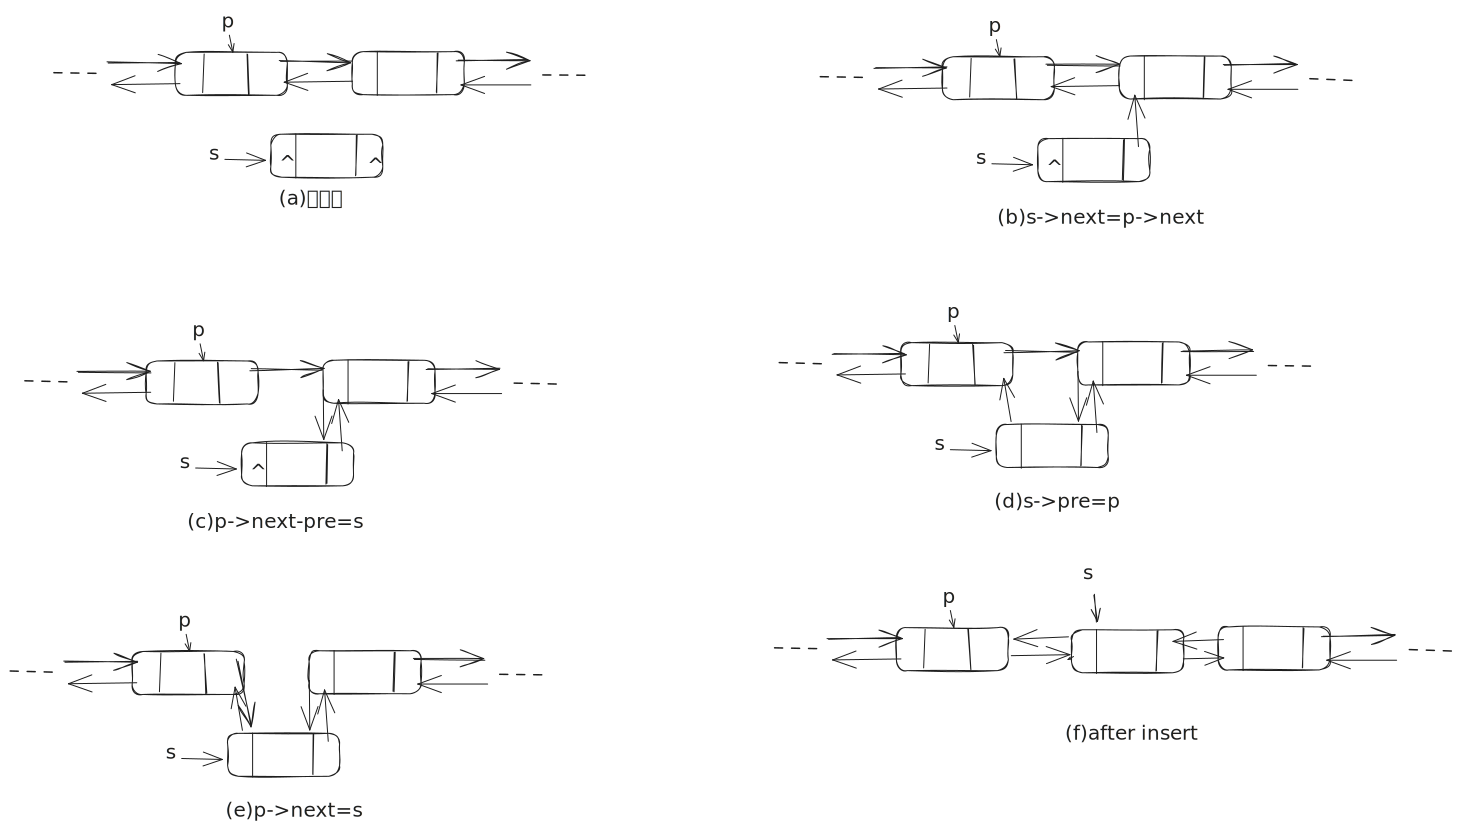
\includegraphics[width=1\textwidth]{./figure/pdf/cropped/insertDL.pdf}
    \caption{p结点之后插入结点s}
    \label{fig:insertAfterDoubleLink}
  \end{figure}
  代码如代码\ref{lst:insertAfterDoubleLink}所示。

  \begin{lstlisting}[language=C++, caption={p结点之后插入结点s示例代码}, label={lst:insertAfterDoubleLink}]
    void insertAfterDoubleLink(DLink* p, DLink* s) {
      s->pre = p;
      s->next = p->next;
      if (p->next != NULL) {
        p->next->pre = s;
      }
      p->next = s;
    }
  \end{lstlisting}

  该算法的总时间复杂度为 $O(1)$,空间复杂度为 $O(1)$。

  特点:在双链表中结点 p 之后插入结点 s。



  \subsubsection{循环链表\textbackslash\&静态链表}
  循环链表是链表的一种,最后一个节点的指针指向第一个节点,形成一个环。
  \textit{示例}:
  $L = \{1001 \rightarrow 1002 \rightarrow 1003 \rightarrow 1001\}$。

  \textbf{循环单链表}:

  循环单链表和单链表的区别在于,循环单链表的尾结点指针指向头结点。

  其结构如图\ref{fig:cycleSingleLink}所示。

  \begin{figure}[h]
    \centering
    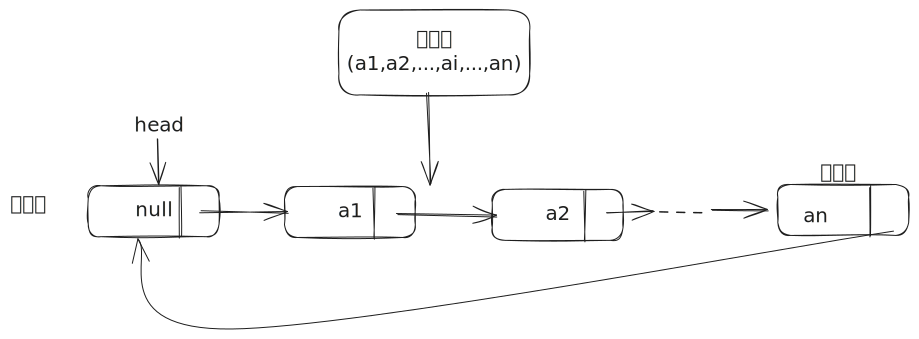
\includegraphics[width=0.6\textwidth]{./figure/pdf/cropped/cycleSLink.pdf}
    \caption{循环单链表结构}
    \label{fig:cycleSingleLink}
  \end{figure}

  \textbf{循环双链表}:

  循环双链表和双链表的区别在于,循环双链表的头结点的前驱指针指向尾结点,尾结点的后继指针指向头结点。

  其结构如图\ref{fig:cycleDoubleLink}所示。

  \begin{figure}[h]
    \centering
    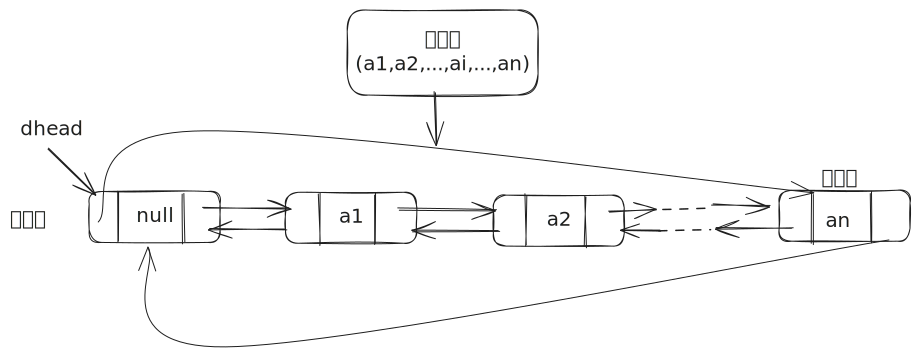
\includegraphics[width=0.6\textwidth]{./figure/pdf/cropped/cycleDLink.pdf}
    \caption{循环双链表结构}
    \label{fig:cycleDoubleLink}
  \end{figure}


  静态链表是使用数组模拟链表的一种实现方式,每个数组元素包含数据域和指针域。与前面所讲的链表不同,静态链表的指针域
  存储的是数组的索引,而不是指向下一个节点的指针。静态链表和顺序表一样,使用数组存储数据元素,但是静态链表可以更好地支持插入和删除操作。

  如图\ref{fig:staticLink}所示,静态链表的结构由数据域和指针域组成,其中数据域存储数据元素,指针域存储数组的索引。

  \begin{figure}[h]
    \centering
    \includegraphics[width=1\textwidth]{./figure/pdf/cropped/staticLink.pdf}
    \caption{静态链表结构}
    \label{fig:staticLink}
  \end{figure}

 数组的第一个元素不存储数据,它的指针域存储第一个数据元素的索引,最后一个元素的指针域存储下一个空闲位置的索引。最后一个
 元素的指针域值为-1。

  \section{顺序表与链表的比较}
  \begin{itemize}
      \item \textbf{存储方式}:顺序表使用数组存储数据元素,链表使用指针存储数据元素。
      \item \textbf{插入和删除}:顺序表插入和删除操作需要移动元素,时间复杂度为 $O(n)$,链表插入和删除操作只需要修改指针,时间复杂度为 $O(1)$。
      \item \textbf{空间复杂度}:顺序表的空间复杂度为 $O(n)$,链表的空间复杂度为 $O(n)$。
      \item \textbf{访问速度}:顺序表的访问速度快,时间复杂度为 $O(1)$,链表的访问速度慢,时间复杂度为 $O(n)$。
  \end{itemize}




\textit{总结}:顺序表适合需要频繁访问的场景,而链表适合需要频繁插入和删除的场景。

\chapter{栈与队列}
从组成元素的逻辑关系来看,栈和队列都属于线性结构.栈和队列与线性表的不同之处在于它们的相关运算具有一些特殊性.
更准确地说,一般线性表上的插入/删除运算不受限制,而栈和队列上的插入 删除运算均会受到某种特殊限制,
因此栈和队列也称为操作受限的线性表.
\section{栈}

\subsection{栈的定义}

栈是一种特殊的线性表,只能在表的一端进行插入和删除操作。栈的插入操作称为入栈,删除操作称为出栈。栈的特点是后进先出,即最后入栈的元素最先出栈。

如图\ref{fig:stack}所示,栈的结构由栈顶和栈底组成,栈顶指向栈顶元素,栈底指向栈底元素。

\begin{figure}[h]
  \centering
  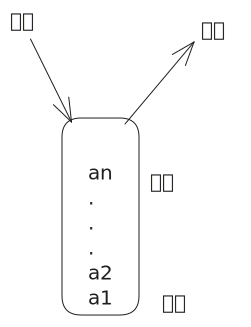
\includegraphics[width=0.4\textwidth]{./figure/pdf/cropped/stack.pdf}
  \caption{栈结构}
  \label{fig:stack}
\end{figure}

相关术语:

\begin{itemize}
  \item \textbf{栈顶}:栈顶是栈中最后一个元素。
  \item \textbf{栈底}:栈底是栈中第一个元素。
  \item \textbf{空栈}:栈中不包含任何元素。
  \item \textbf{满栈}:栈中包含的元素个数等于栈的最大容量。
  \item \textbf{栈的大小}:栈中包含的元素个数。
  \item \textbf{栈的容量}:栈的最大容量。
  \item \textbf{栈的压入}:将元素压入栈中。
  \item \textbf{栈的弹出}:将元素从栈中弹出。
  \end{itemize}

栈的特点:

\begin{itemize}
  \item 栈是一种特殊的线性表,只能在表的一端进行插入和删除操作。
  \item 栈的插入操作称为入栈,删除操作称为出栈。
  \item 栈的特点是后进先出,即最后入栈的元素最先出栈。
\end{itemize}
\subsection{栈的操作}

栈的基本操作包括创建、销毁、压入、弹出、获取栈顶元素、判断栈是否为空、判断栈是否为满、获取栈的大小和获取栈的容量。

\begin{itemize}
  \item \textbf{创建操作}:创建一个空栈。
  \item \textbf{销毁操作}:销毁栈。
  \item \textbf{压入操作}:将元素压入栈中。
  \item \textbf{弹出操作}:将元素从栈中弹出。
  \item \textbf{获取栈顶元素}:获取栈顶元素。
  \item \textbf{判断栈是否为空}:判断栈中是否包含元素。
  \item \textbf{判断栈是否为满}:判断栈中是否包含元素。
  \item \textbf{获取栈的大小}:获取栈中包含的元素个数。
  \item \textbf{获取栈的容量}:获取栈的最大容量。
  \item \textbf{清空栈}:清空栈中的所有元素。
  \item \textbf{遍历栈}:遍历栈中的所有元素。
\end{itemize}


\subsection{顺序栈}

顺序栈是使用数组实现的栈,栈的大小是固定的,栈的容量是数组的大小。

顺序栈的结构体定义如代码\ref{lst:seqStackStruct}所示。

\begin{lstlisting}[language=C++, caption={顺序栈结构体定义}, label={lst:seqStackStruct}]
  struct SeqStack {
    int* data;//栈的数据元素
    int top;//栈顶指针
    int capacity;//栈的容量
  };
\end{lstlisting}

顺序栈的存放过程如图\ref{fig:seqStack}所示。

\begin{figure}[h]
  \centering
  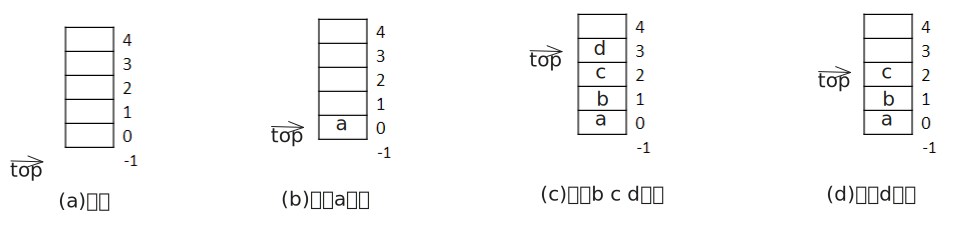
\includegraphics[width=1\textwidth]{./figure/pdf/cropped/processOfSeqStack.pdf}
  \caption{顺序栈存放过程}
  \label{fig:seqStack}
\end{figure}

顺序栈的基本操作包括创建、销毁、压入、弹出、获取栈顶元素、判断栈是否为空、判断栈是否为满、获取栈的大小和获取栈的容量。

\textbf{创建操作}:

创建一个空的顺序栈,需要为栈分配内存空间,并初始化栈的大小、栈的容量和栈顶指针。

代码如代码\ref{lst:createSeqStack}所示。

\begin{lstlisting}[language=C++, caption={创建一个空顺序栈示例代码}, label={lst:createSeqStack}]
  SeqStack* createSeqStack(int capacity) {
    SeqStack* S = (SeqStack*)malloc(sizeof(SeqStack));
    S->data = (int*)malloc(sizeof(int) * capacity);
    S->top = -1;
    S->capacity = capacity;
    return S;
  }

\end{lstlisting}

该算法的总时间复杂度为 $O(1)$,空间复杂度为 $O(n)$。

特点:创建的顺序栈为空,不包含任何数据元素。

\textbf{销毁操作}:

销毁顺序栈,需要释放栈的内存空间。

代码如代码\ref{lst:destroySeqStack}所示。

\begin{lstlisting}[language=C++, caption={销毁顺序栈示例代码}, label={lst:destroySeqStack}]
  void destroySeqStack(SeqStack* S) {
    free(S->data);
    free(S);
  }
\end{lstlisting}

该算法的总时间复杂度为 $O(1)$,空间复杂度为 $O(1)$。

特点:销毁顺序栈,释放栈的内存空间。

\textbf{判满操作}:

判断顺序栈是否为满,即栈中包含的元素个数等于栈的容量。

代码如代码\ref{lst:isFullSeqStack}所示。

\begin{lstlisting}[language=C++, caption={判断顺序栈是否为满示例代码}, label={lst:isFullSeqStack}]
  bool isFullSeqStack(SeqStack* S) {
    return S->top == S->capacity - 1;
  }

\end{lstlisting}

该算法的总时间复杂度为 $O(1)$,空间复杂度为 $O(1)$。

特点:判断顺序栈是否为满,即栈中包含的元素个数等于栈的容量。

\textbf{判空操作}:

判断顺序栈是否为空,即栈中不包含任何元素。

代码如代码\ref{lst:isEmptySeqStack}所示。

\begin{lstlisting}[language=C++, caption={判断顺序栈是否为空示例代码}, label={lst:isEmptySeqStack}]
  bool isEmptySeqStack(SeqStack* S) {
    return S->top == -1;
  }

\end{lstlisting}

该算法的总时间复杂度为 $O(1)$,空间复杂度为 $O(1)$。

特点:判断顺序栈是否为空,即栈中不包含任何元素。

\textbf{压入操作}:

将元素压入顺序栈中,即将元素放入栈顶。

代码如代码\ref{lst:pushSeqStack}所示。

\begin{lstlisting}[language=C++, caption={压入顺序栈示例代码}, label={lst:pushSeqStack}]
  void pushSeqStack(SeqStack* S, int data) {
    if (isFullSeqStack(S)) {
      printf("栈已满,无法压入元素\n");
      return;
    }
    S->data[++S->top] = data;
  }

\end{lstlisting}

该算法的总时间复杂度为 $O(1)$,空间复杂度为 $O(1)$。

特点:将元素压入顺序栈中,即将元素放入栈顶。

\textbf{弹出操作}:

将元素从顺序栈中弹出,即将栈顶元素删除。

代码如代码\ref{lst:popSeqStack}所示。

\begin{lstlisting}[language=C++, caption={弹出顺序栈示例代码}, label={lst:popSeqStack}]
  void popSeqStack(SeqStack* S) {
    if (isEmptySeqStack(S)) {
      printf("栈为空,无法弹出元素\n");
      return;
    }
    S->top--;
  }

\end{lstlisting}

该算法的总时间复杂度为 $O(1)$,空间复杂度为 $O(1)$。

特点:将元素从顺序栈中弹出,即将栈顶元素删除。

\textbf{获取栈顶元素}:

获取顺序栈的栈顶元素,即获取栈顶元素的值。

代码如代码\ref{lst:getTopSeqStack}所示。

\begin{lstlisting}[language=C++, caption={获取顺序栈的栈顶元素示例代码}, label={lst:getTopSeqStack}]
  int getTopSeqStack(SeqStack* S) {
    if (isEmptySeqStack(S)) {
      printf("栈为空,无法获取栈顶元素\n");
      return -1;
    }
    return S->data[S->top];
  }

\end{lstlisting}

该算法的总时间复杂度为 $O(1)$,空间复杂度为 $O(1)$。

特点:获取顺序栈的栈顶元素,即获取栈顶元素的值。

\textbf{获取栈的大小}:

获取顺序栈的大小,即获取栈中包含的元素个数。

代码如代码\ref{lst:sizeSeqStack}所示。

\begin{lstlisting}[language=C++, caption={获取顺序栈的大小示例代码}, label={lst:sizeSeqStack}]
  int sizeSeqStack(SeqStack* S) {
    return S->top + 1;
  }

\end{lstlisting}

该算法的总时间复杂度为 $O(1)$,空间复杂度为 $O(1)$。

特点:获取顺序栈的大小,即获取栈中包含的元素个数。

\textbf{获取栈的容量}:

获取顺序栈的容量,即获取栈的最大容量。

代码如代码\ref{lst:capacitySeqStack}所示。

\begin{lstlisting}[language=C++, caption={获取顺序栈的容量示例代码}, label={lst:capacitySeqStack}]
  int capacitySeqStack(SeqStack* S) {
    return S->capacity;
  }

\end{lstlisting}

该算法的总时间复杂度为 $O(1)$,空间复杂度为 $O(1)$。

特点:获取顺序栈的容量,即获取栈的最大容量。

\textbf{清空栈}:

清空顺序栈,即将栈中的所有元素删除。

代码如代码\ref{lst:clearSeqStack}所示。

\begin{lstlisting}[language=C++, caption={清空顺序栈示例代码}, label={lst:clearSeqStack}]
  void clearSeqStack(SeqStack* S) {
    S->top = -1;
  }

\end{lstlisting}

该算法的总时间复杂度为 $O(1)$,空间复杂度为 $O(1)$。

特点:清空顺序栈,即将栈中的所有元素删除。

\textbf{遍历栈}:

遍历顺序栈,即输出栈中的所有元素。

代码如代码\ref{lst:traverseSeqStack}所示。

\begin{lstlisting}[language=C++, caption={遍历顺序栈示例代码}, label={lst:traverseSeqStack}]
  void traverseSeqStack(SeqStack* S) {
    for (int i = 0; i <= S->top; i++) {
      printf("%d ", S->data[i]);
    }
    printf("\n");
  }

\end{lstlisting}

该算法的总时间复杂度为 $O(n)$,空间复杂度为 $O(1)$。

特点:遍历顺序栈,即输出栈中的所有元素。




\subsection{链栈}

栈是线性表的特例,线性表的存储结构还有链式存储结构,因此栈也可以使用链式存储结构实现,称为链栈.

链栈的结构体定义如代码\ref{lst:linkStackStruct}所示。

\begin{lstlisting}[language=C++, caption={链栈结构体定义}, label={lst:linkStackStruct}]
  struct LinkStack {
    int data;//栈的数据元素
    LinkStack* next;//栈的下一个元素
  };
\end{lstlisting}

链栈结构如图\ref{fig:linkStack}所示。

\begin{figure}[h]
  \centering
  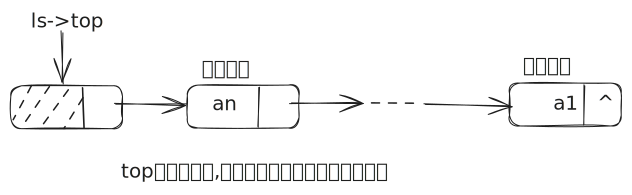
\includegraphics[width=1\textwidth]{./figure/pdf/cropped/linkStack.pdf}
  \caption{链栈}
  \label{fig:linkStack}
\end{figure}

我们可以发现,链栈的结构与单链表的结构相似,只是链栈的操作受到了限制,只能在栈顶进行插入和删除操作。

链栈的基本操作包括创建、销毁、压入、弹出、获取栈顶元素、判断栈是否为空、获取栈的大小和遍历栈。

\textbf{创建操作}:

创建一个空链栈,需要为栈分配内存空间,并初始化栈顶指针。

代码如代码\ref{lst:createLinkStack}所示。

\begin{lstlisting}[language=C++, caption={创建一个空链栈示例代码}, label={lst:createLinkStack}]
  LinkStack* createLinkStack() {
    LinkStack* S = (LinkStack*)malloc(sizeof(LinkStack));
    S->next = NULL;
    return S;
  }

\end{lstlisting}

该算法的总时间复杂度为 $O(1)$,空间复杂度为 $O(1)$。

特点:创建的链栈为空,不包含任何数据元素。

\textbf{销毁操作}:

销毁链栈,需要释放栈的内存空间。

代码如代码\ref{lst:destroyLinkStack}所示。

\begin{lstlisting}[language=C++, caption={销毁链栈示例代码}, label={lst:destroyLinkStack}]
  void destroyLinkStack(LinkStack* S) {
    LinkStack* p = S;
    while (p != NULL) {
      LinkStack* q = p;
      p = p->next;
      free(q);
    }
  }

\end{lstlisting}

该算法的总时间复杂度为 $O(n)$,空间复杂度为 $O(1)$。

特点:销毁链栈,释放栈的内存空间。

\textbf{判空操作}:

判断链栈是否为空,即栈中不包含任何元素。

代码如代码\ref{lst:isEmptyLinkStack}所示。

\begin{lstlisting}[language=C++, caption={判断链栈是否为空示例代码}, label={lst:isEmptyLinkStack}]
  bool isEmptyLinkStack(LinkStack* S) {
    return S->next == NULL;
  }

\end{lstlisting}

该算法的总时间复杂度为 $O(1)$,空间复杂度为 $O(1)$。

特点:判断链栈是否为空,即栈中不包含任何元素。

\textbf{压入操作}:

将元素压入链栈中,即将元素放入栈顶。

代码如代码\ref{lst:pushLinkStack}所示。

\begin{lstlisting}[language=C++, caption={压入链栈示例代码}, label={lst:pushLinkStack}]
  void pushLinkStack(LinkStack* S, int data) {
    LinkStack* p = (LinkStack*)malloc(sizeof(LinkStack));
    p->data = data;
    p->next = S->next;
    S->next = p;
  }

\end{lstlisting}

该算法的总时间复杂度为 $O(1)$,空间复杂度为 $O(1)$。

特点:将元素压入链栈中,即将元素放入栈顶。

\textbf{弹出操作}:

将元素从链栈中弹出,即将栈顶元素删除。

代码如代码\ref{lst:popLinkStack}所示。

\begin{lstlisting}[language=C++, caption={弹出链栈示例代码}, label={lst:popLinkStack}]
  void popLinkStack(LinkStack* S) {
    if (isEmptyLinkStack(S)) {
      printf("栈为空,无法弹出元素\n");
      return;
    }
    LinkStack* p = S->next;
    S->next = p->next;
    free(p);
  }

\end{lstlisting}

该算法的总时间复杂度为 $O(1)$,空间复杂度为 $O(1)$。

特点:将元素从链栈中弹出,即将栈顶元素删除。

\textbf{获取栈顶元素}:

获取链栈的栈顶元素,即获取栈顶元素的值。

代码如代码\ref{lst:getTopLinkStack}所示。

\begin{lstlisting}[language=C++, caption={获取链栈的栈顶元素示例代码}, label={lst:getTopLinkStack}]
  int getTopLinkStack(LinkStack* S) {
    if (isEmptyLinkStack(S)) {
      printf("栈为空,无法获取栈顶元素\n");
      return -1;
    }
    return S->next->data;
  }

\end{lstlisting}

该算法的总时间复杂度为 $O(1)$,空间复杂度为 $O(1)$。

特点:获取链栈的栈顶元素,即获取栈顶元素的值。

\textbf{遍历栈}:

遍历链栈,即输出栈中的所有元素。

代码如代码\ref{lst:traverseLinkStack}所示。

\begin{lstlisting}[language=C++, caption={遍历链栈示例代码}, label={lst:traverseLinkStack}]
  void traverseLinkStack(LinkStack* S) {
    LinkStack* p = S->next;
    while (p != NULL) {
      printf("%d ", p->data);
      p = p->next;
    }
    printf("\n");
  }

\end{lstlisting}

该算法的总时间复杂度为 $O(n)$,空间复杂度为 $O(1)$。

特点:遍历链栈,即输出栈中的所有元素。



\subsection{共享栈}

共享栈是两个栈共享一个存储空间的栈,两个栈的栈底分别位于共享空间的两端,两个栈的栈顶向中间延伸。

共享栈的结构如图\ref{fig:sharedStack}所示。

\begin{figure}[h]
  \centering
  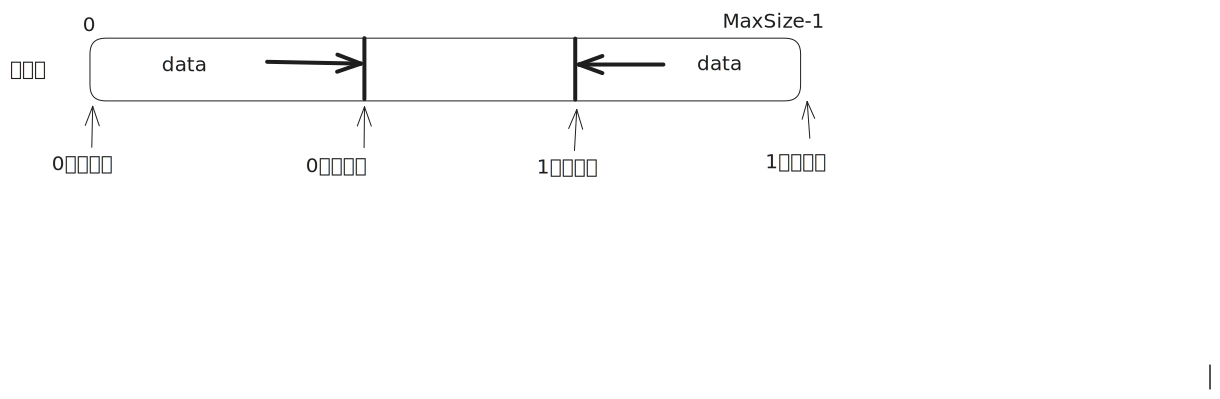
\includegraphics[width=1\textwidth]{./figure/pdf/cropped/shareStack.pdf}
  \caption{共享栈}
  \label{fig:sharedStack}
\end{figure}


共享栈的结构体定义如代码\ref{lst:sharedStackStruct}所示。

\begin{lstlisting}[language=C++, caption={共享栈结构体定义}, label={lst:sharedStackStruct}]
  struct SharedStack {
    int* data;//栈的数据元素
    int top1;//栈1的栈顶指针
    int top2;//栈2的栈顶指针
    int capacity;//栈的容量
  };
\end{lstlisting}

共享栈的基本操作包括创建、销毁、压入、弹出、获取栈顶元素、判断栈是否为空、判断栈是否为满、获取栈的大小和获取栈的容量。

\textbf{创建操作}:

创建一个空共享栈,需要为栈分配内存空间,并初始化栈的大小、栈的容量和栈顶指针。

代码如代码\ref{lst:createSharedStack}所示。

\begin{lstlisting}[language=C++, caption={创建一个空共享栈示例代码}, label={lst:createSharedStack}]
  SharedStack* createSharedStack(int capacity) {
    SharedStack* S = (SharedStack*)malloc(sizeof(SharedStack));
    S->data = (int*)malloc(sizeof(int) * capacity);
    S->top1 = -1;
    S->top2 = capacity;
    S->capacity = capacity;
    return S;
  }

\end{lstlisting}

该算法的总时间复杂度为 $O(1)$,空间复杂度为 $O(1)$。

特点:创建的共享栈为空,不包含任何数据元素。

\textbf{销毁操作}:

销毁共享栈,需要释放栈的内存空间。

代码如代码\ref{lst:destroySharedStack}所示。

\begin{lstlisting}[language=C++, caption={销毁共享栈示例代码}, label={lst:destroySharedStack}]
  void destroySharedStack(SharedStack* S) {
    free(S->data);
    free(S);
  }

\end{lstlisting}

该算法的总时间复杂度为 $O(1)$,空间复杂度为 $O(1)$。

特点:销毁共享栈,释放栈的内存空间。

\textbf{判空操作}:

判断共享栈是否为空,即栈中不包含任何元素。

代码如代码\ref{lst:isEmptySharedStack}所示。

\begin{lstlisting}[language=C++, caption={判断共享栈是否为空示例代码}, label={lst:isEmptySharedStack}]
  bool isEmptySharedStack(SharedStack* S, int stackNumber) {
    if (stackNumber == 1) {
      return S->top1 == -1;
    } else if (stackNumber == 2) {
      return S->top2 == S->capacity;
    } else {
      return false;
    }
  }

\end{lstlisting}

该算法的总时间复杂度为 $O(1)$,空间复杂度为 $O(1)$。

特点:判断共享栈是否为空,即栈中不包含任何元素。

\textbf{判满操作}:

判断共享栈是否为满,即栈中包含的元素个数等于栈的容量。

代码如代码\ref{lst:isFullSharedStack}所示。

\begin{lstlisting}[language=C++, caption={判断共享栈是否为满示例代码}, label={lst:isFullSharedStack}]
  bool isFullSharedStack(SharedStack* S) {
    return S->top1 + 1 == S->top2;
  }

\end{lstlisting}

该算法的总时间复杂度为 $O(1)$,空间复杂度为 $O(1)$。

特点:判断共享栈是否为满,即栈中包含的元素个数等于栈的容量。

\textbf{压入操作}:

将元素压入共享栈中,即将元素放入栈顶。

代码如代码\ref{lst:pushSharedStack}所示。

\begin{lstlisting}[language=C++, caption={压入共享栈示例代码}, label={lst:pushSharedStack}]
  void pushSharedStack(SharedStack* S, int data, int stackNumber) {
    if (isFullSharedStack(S)) {
      printf("栈已满,无法压入元素\n");
      return;
    }
    if (stackNumber == 1) {
      S->data[++S->top1] = data;
    } else if (stackNumber == 2) {
      S->data[--S->top2] = data;
    }
  }

\end{lstlisting}

该算法的总时间复杂度为 $O(1)$,空间复杂度为 $O(1)$。

特点:将元素压入共享栈中,即将元素放入栈顶。

\textbf{弹出操作}:

将元素从共享栈中弹出,即将栈顶元素删除。

代码如代码\ref{lst:popSharedStack}所示。

\begin{lstlisting}[language=C++, caption={弹出共享栈示例代码}, label={lst:popSharedStack}]
  void popSharedStack(SharedStack* S, int stackNumber) {
    if (isEmptySharedStack(S, stackNumber)) {
      printf("栈为空,无法弹出元素\n");
      return;
    }
    if (stackNumber == 1) {
      S->top1--;
    } else if (stackNumber == 2) {
      S->top2++;
    }
  }

\end{lstlisting}

该算法的总时间复杂度为 $O(1)$,空间复杂度为 $O(1)$。

特点:将元素从共享栈中弹出,即将栈顶元素删除。

\textbf{获取栈顶元素}:

获取共享栈的栈顶元素,即获取栈顶元素的值。

代码如代码\ref{lst:getTopSharedStack}所示。

\begin{lstlisting}[language=C++, caption={获取共享栈的栈顶元素示例代码}, label={lst:getTopSharedStack}]
  int getTopSharedStack(SharedStack* S, int stackNumber) {
    if (isEmptySharedStack(S, stackNumber)) {
      printf("栈为空,无法获取栈顶元素\n");
      return -1;
    }
    if (stackNumber == 1) {
      return S->data[S->top1];
    } else if (stackNumber == 2) {
      return S->data[S->top2];
    } else {
      return -1;
    }
  }

\end{lstlisting}

该算法的总时间复杂度为 $O(1)$,空间复杂度为 $O(1)$。

特点:获取共享栈的栈顶元素,即获取栈顶元素的值。

\textbf{获取栈的大小}:

获取共享栈的大小,即获取栈中包含的元素个数。

代码如代码\ref{lst:sizeSharedStack}所示。

\begin{lstlisting}[language=C++, caption={获取共享栈的大小示例代码}, label={lst:sizeSharedStack}]
  int sizeSharedStack(SharedStack* S) {
    return S->top1 + 1 + S->capacity - S->top2;
  }

\end{lstlisting}

该算法的总时间复杂度为 $O(1)$,空间复杂度为 $O(1)$。

特点:获取共享栈的大小,即获取栈中包含的元素个数。

\textbf{获取栈的容量}:

获取共享栈的容量,即获取栈的最大容量。

代码如代码\ref{lst:capacitySharedStack}所示。

\begin{lstlisting}[language=C++, caption={获取共享栈的容量示例代码}, label={lst:capacitySharedStack}]
  int capacitySharedStack(SharedStack* S) {
    return S->capacity;
  }

\end{lstlisting}

该算法的总时间复杂度为 $O(1)$,空间复杂度为 $O(1)$。

特点:获取共享栈的容量,即获取栈的最大容量。

\textbf{清空栈}:

清空共享栈,即将栈中的所有元素删除。

代码如代码\ref{lst:clearSharedStack}所示。

\begin{lstlisting}[language=C++, caption={清空共享栈示例代码}, label={lst:clearSharedStack}]
  void clearSharedStack(SharedStack* S) {
    S->top1 = -1;
    S->top2 = S->capacity;
  }

\end{lstlisting}

该算法的总时间复杂度为 $O(1)$,空间复杂度为 $O(1)$。

特点:清空共享栈,即将栈中的所有元素删除。

\textbf{遍历栈}:

遍历共享栈,即输出栈中的所有元素。

代码如代码\ref{lst:traverseSharedStack}所示。

\begin{lstlisting}[language=C++, caption={遍历共享栈示例代码}, label={lst:traverseSharedStack}]
  void traverseSharedStack(SharedStack* S) {
    for (int i = 0; i <= S->top1; i++) {
      printf("%d ", S->data[i]);
    }
    for (int i = S->capacity - 1; i >= S->top2; i--) {
      printf("%d ", S->data[i]);
    }
    printf("\n");
  }

\end{lstlisting}

该算法的总时间复杂度为 $O(n)$,空间复杂度为 $O(1)$。

特点:遍历共享栈,即输出栈中的所有元素。


\section{队列}



\subsection{队列的定义}

队列是一种先进先出的线性表,只允许在表的一端进行插入,而在另一端进行删除操作。


\subsection{队列的操作}

队列的基本操作包括创建、销毁、入队、出队、获取队头元素、判断队列是否为空、判断队列是否为满、获取队列的大小和获取队列的容量。


\subsection{顺序队列}

顺序队列是使用数组实现的队列,队列的大小是固定的,队列的容量是数组的大小。

顺序队列的结构如如图\ref{fig:seqQueue}所示。

\begin{figure}[h]
  \centering
  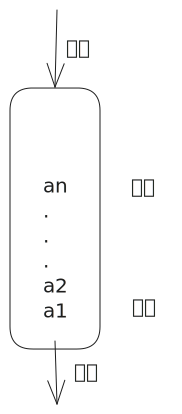
\includegraphics[width=0.1\textwidth]{./figure/pdf/cropped/seqQueue.pdf}
  \caption{顺序队列}
  \label{fig:seqQueue}
\end{figure}

顺序队列的结构体定义如代码\ref{lst:seqQueueStruct}所示。

\begin{lstlisting}[language=C++, caption={顺序队列结构体定义}, label={lst:seqQueueStruct}]
  struct SeqQueue {
    int* data;//队列的数据元素
    int front;//队头指针
    int rear;//队尾指针
    int capacity;//队列的容量
  };
\end{lstlisting}

顺序队列的存放过程如图\ref{fig:seqQueuePut}所示。

\begin{figure}[h]
  \centering
  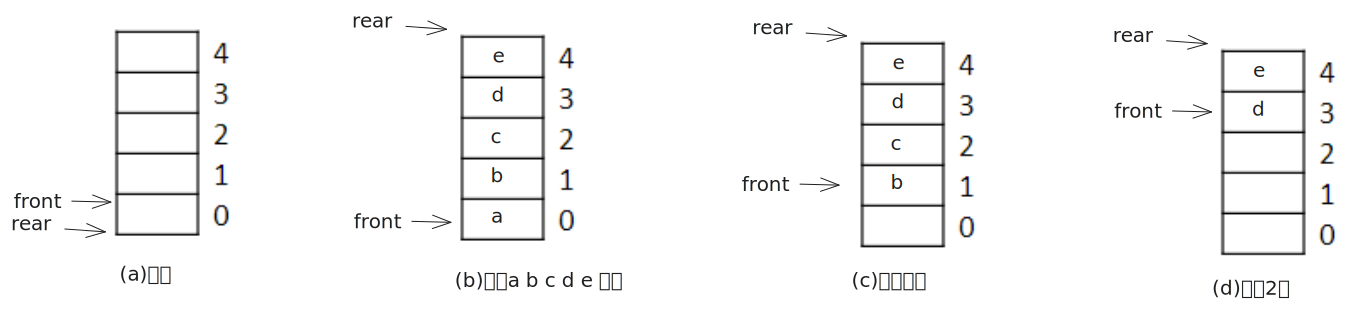
\includegraphics[width=1\textwidth]{./figure/pdf/cropped/seqQueuePut.pdf}
  \caption{顺序队列的存放过程}
  \label{fig:seqQueuePut}
\end{figure}

相关术语:

\begin{itemize}
  \item 队头指针:指向队头元素的前一个位置。
  \item 队尾指针:指向队尾元素。
  \item 队列的容量:队列的最大容量。
  \item 队列的大小:队列中包含的元素个数。
  \item 队列的长度:队列中包含的元素个数。
  \item 队列的空间:队列的容量减去队列的大小。
  \item 队列的空:队列的大小为0。
  \item 队列的满:队列的大小等于队列的容量。
\end{itemize}

顺序队列的基本操作包括创建、销毁、入队、出队、获取队头元素、判断队列是否为空、判断队列是否为满、获取队列的大小和获取队列的容量。

\textbf{创建操作}:

创建一个空顺序队列,需要为队列分配内存空间,并初始化队头指针、队尾指针和队列的容量。

代码如代码\ref{lst:createSeqQueue}所示。

\begin{lstlisting}[language=C++, caption={创建一个空顺序队列示例代码}, label={lst:createSeqQueue}]
  SeqQueue* createSeqQueue(int capacity) {
    SeqQueue* Q = (SeqQueue*)malloc(sizeof(SeqQueue));
    Q->data = (int*)malloc(sizeof(int) * capacity);
    Q->front = 0;
    Q->rear = 0;
    Q->capacity = capacity;
    return Q;
  }

\end{lstlisting}

该算法的总时间复杂度为 $O(1)$,空间复杂度为 $O(1)$。

特点:创建的顺序队列为空,不包含任何数据元素。

\textbf{销毁操作}:

销毁顺序队列,需要释放队列的内存空间。

代码如代码\ref{lst:destroySeqQueue}所示。

\begin{lstlisting}[language=C++, caption={销毁顺序队列示例代码}, label={lst:destroySeqQueue}]
  void destroySeqQueue(SeqQueue* Q) {
    free(Q->data);
    free(Q);
  }

\end{lstlisting}

该算法的总时间复杂度为 $O(1)$,空间复杂度为 $O(1)$。

特点:销毁顺序队列,释放队列的内存空间。

\textbf{判空操作}:

判断顺序队列是否为空,即队列中不包含任何元素。

代码如代码\ref{lst:isEmptySeqQueue}所示。

\begin{lstlisting}[language=C++, caption={判断顺序队列是否为空示例代码}, label={lst:isEmptySeqQueue}]
  bool isEmptySeqQueue(SeqQueue* Q) {
    return Q->front == Q->rear;
  }

\end{lstlisting}

该算法的总时间复杂度为 $O(1)$,空间复杂度为 $O(1)$。

特点:判断顺序队列是否为空,即队列中不包含任何元素。

\textbf{判满操作}:

判断顺序队列是否为满,即队列中包含的元素个数等于队列的容量。

代码如代码\ref{lst:isFullSeqQueue}所示。

\begin{lstlisting}[language=C++, caption={判断顺序队列是否为满示例代码}, label={lst:isFullSeqQueue}]
  bool isFullSeqQueue(SeqQueue* Q) {
    return (Q->rear + 1) % Q->capacity == Q->front;
  }

\end{lstlisting}

该算法的总时间复杂度为 $O(1)$,空间复杂度为 $O(1)$。

特点:判断顺序队列是否为满,即队列中包含的元素个数等于队列的容量。

\textbf{入队操作}:

将元素入队,即将元素放入队尾。

代码如代码\ref{lst:enQueueSeqQueue}所示。

\begin{lstlisting}[language=C++, caption={入队示例代码}, label={lst:enQueueSeqQueue}]
  void enQueueSeqQueue(SeqQueue* Q, int data) {
    if (isFullSeqQueue(Q)) {
      printf("队列已满,无法入队\n");
      return;
    }
    Q->data[Q->rear] = data;
    Q->rear = (Q->rear + 1) % Q->capacity;
  }

\end{lstlisting}

该算法的总时间复杂度为 $O(1)$,空间复杂度为 $O(1)$。

特点:将元素入队,即将元素放入队尾。

\textbf{出队操作}:

将元素出队,即将队头元素删除。

代码如代码\ref{lst:deQueueSeqQueue}所示。

\begin{lstlisting}[language=C++, caption={出队示例代码}, label={lst:deQueueSeqQueue}]
  void deQueueSeqQueue(SeqQueue* Q) {
    if (isEmptySeqQueue(Q)) {
      printf("队列为空,无法出队\n");
      return;
    }
    Q->front = (Q->front + 1) % Q->capacity;
  }

\end{lstlisting}

该算法的总时间复杂度为 $O(1)$,空间复杂度为 $O(1)$。

特点:将元素出队,即将队头元素删除。

\textbf{获取队头元素}:

获取顺序队列的队头元素,即获取队头元素的值。

代码如代码\ref{lst:getFrontSeqQueue}所示。

\begin{lstlisting}[language=C++, caption={获取队头元素示例代码}, label={lst:getFrontSeqQueue}]
  int getFrontSeqQueue(SeqQueue* Q) {
    if (isEmptySeqQueue(Q)) {
      printf("队列为空,无法获取队头元素\n");
      return -1;
    }
    return Q->data[Q->front];
  }

\end{lstlisting}

该算法的总时间复杂度为 $O(1)$,空间复杂度为 $O(1)$。

特点:获取顺序队列的队头元素,即获取队头元素的值。

\textbf{获取队列的大小}:

获取顺序队列的大小,即获取队列中包含的元素个数。

代码如代码\ref{lst:sizeSeqQueue}所示。

\begin{lstlisting}[language=C++, caption={获取队列的大小示例代码}, label={lst:sizeSeqQueue}]
  int sizeSeqQueue(SeqQueue* Q) {
    return (Q->rear - Q->front + Q->capacity) % Q->capacity;
  }

\end{lstlisting}

该算法的总时间复杂度为 $O(1)$,空间复杂度为 $O(1)$。

特点:获取顺序队列的大小,即获取队列中包含的元素个数。

\textbf{获取队列的容量}:

获取顺序队列的容量,即获取队列的最大容量。

代码如代码\ref{lst:capacitySeqQueue}所示。

\begin{lstlisting}[language=C++, caption={获取队列的容量示例代码}, label={lst:capacitySeqQueue}]
  int capacitySeqQueue(SeqQueue* Q) {
    return Q->capacity;
  }

\end{lstlisting}

该算法的总时间复杂度为 $O(1)$,空间复杂度为 $O(1)$。

特点:获取顺序队列的容量,即获取队列的最大容量。

\textbf{清空队列}:

清空顺序队列,即将队列中的所有元素删除。

代码如代码\ref{lst:clearSeqQueue}所示。

\begin{lstlisting}[language=C++, caption={清空队列示例代码}, label={lst:clearSeqQueue}]
  void clearSeqQueue(SeqQueue* Q) {
    Q->front = 0;
    Q->rear = 0;
  }

\end{lstlisting}

该算法的总时间复杂度为 $O(1)$,空间复杂度为 $O(1)$。

特点:清空顺序队列,即将队列中的所有元素删除。

\textbf{遍历队列}:

遍历顺序队列,即输出队列中的所有元素。

代码如代码\ref{lst:traverseSeqQueue}所示。

\begin{lstlisting}[language=C++, caption={遍历队列示例代码}, label={lst:traverseSeqQueue}]
  void traverseSeqQueue(SeqQueue* Q) {
    for (int i = Q->front; i != Q->rear; i = (i + 1) % Q->capacity) {
      printf("%d ", Q->data[i]);
    }
    printf("\n");
  }

\end{lstlisting}

该算法的总时间复杂度为 $O(n)$,空间复杂度为 $O(1)$。

特点:遍历顺序队列,即输出队列中的所有元素。

针对循环队列,我们还可以使用另外两种方法来判断队列是否为空和队列是否为满。

第一种:使用一个变量记录队列的大小,当队列为空时,队列的大小为0;当队列为满时,队列的大小等于队列的容量。

第二种:新增一个tag变量,当队列为空时,tag等于0;当队列为满时,tag等于1。
第一种的结构体为:

\begin{lstlisting}[language=C++, caption={循环队列结构体定义}, label={lst:circleQueueStruct}]
  struct CircleQueue {
    int* data;//队列的数据元素
    int front;//队头指针
    int rear;//队尾指针
    int size;//队列的大小
    int capacity;//队列的容量
  };
\end{lstlisting}

\textbf{判空操作}:

判断循环队列是否为空,即队列中不包含任何元素。

代码如代码\ref{lst:isEmptyCircleQueue}所示。

\begin{lstlisting}[language=C++, caption={判断循环队列是否为空示例代码}, label={lst:isEmptyCircleQueue}]
  bool isEmptyCircleQueue(CircleQueue* Q) {
    return Q->size == 0;
  }

\end{lstlisting}

\textbf{判满操作}:

判断循环队列是否为满,即队列中包含的元素个数等于队列的容量。

代码如代码\ref{lst:isFullCircleQueue}所示。

\begin{lstlisting}[language=C++, caption={判断循环队列是否为满示例代码}, label={lst:isFullCircleQueue}]
  bool isFullCircleQueue(CircleQueue* Q) {
    return Q->size == Q->capacity;
  }

\end{lstlisting}

第二种的结构体为:

\begin{lstlisting}[language=C++, caption={循环队列结构体定义}, label={lst:circleQueueStruct}]
  struct CircleQueue {
    int* data;//队列的数据元素
    int front;//队头指针
    int rear;//队尾指针
    int tag;//标记队列是否为满
    int capacity;//队列的容量
  };
\end{lstlisting}

\textbf{判空操作}:

判断循环队列是否为空,即队列中不包含任何元素。

代码如代码\ref{lst:isEmptyCircleQueue}所示。

\begin{lstlisting}[language=C++, caption={判断循环队列是否为空示例代码}, label={lst:isEmptyCircleQueue}]
  bool isEmptyCircleQueue(CircleQueue* Q) {
    return Q->front == Q->rear && Q->tag == 0;
  }

\end{lstlisting}

\textbf{判满操作}:

判断循环队列是否为满,即队列中包含的元素个数等于队列的容量。

代码如代码\ref{lst:isFullCircleQueue}所示。

\begin{lstlisting}[language=C++, caption={判断循环队列是否为满示例代码}, label={lst:isFullCircleQueue}]
  bool isFullCircleQueue(CircleQueue* Q) {
    return Q->front == Q->rear && Q->tag == 1;
  }

\end{lstlisting}

\subsection{链式队列}

链式队列是使用链表实现的队列,队列的大小是动态的,队列的容量是无限的。

链式队列的结构如如图\ref{fig:linkQueue}所示。

\begin{figure}[h]
  \centering
  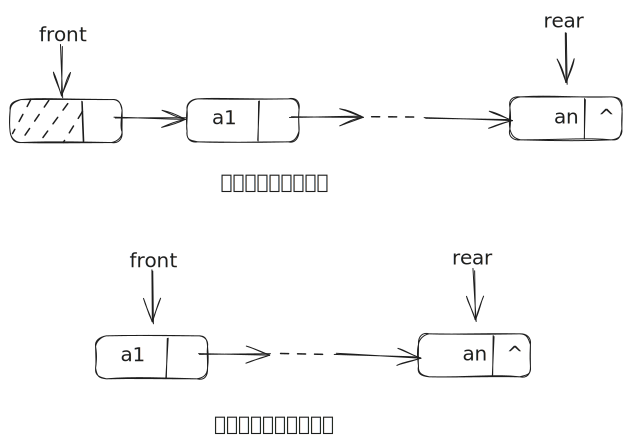
\includegraphics[width=1\textwidth]{./figure/pdf/cropped/linkQueue.pdf}
  \caption{链式队列}
  \label{fig:linkQueue}
\end{figure}

图中示出了两类链式队列,一类带头结点,一类不带头结点。

我们可以发现,不带头结点的链式队列需要特殊处理队列为空的情况,因为队列为空时,
队头指针和队尾指针都为空。因此,我们通常使用带头结点的链式队列。

链式队列的结构体定义如代码\ref{lst:linkQueueStruct}所示。

\begin{lstlisting}[language=C++, caption={链式队列结构体定义}, label={lst:linkQueueStruct}]
  struct singleLink {
	NODETYPE data;
	singleLink* next;
  }; 
  struct LinkQueue {
    singleLink* front, * rear;
  };
\end{lstlisting}

链式队列的基本操作包括创建、销毁、入队、出队、获取队头元素、判断队列是否为空、获取队列的大小。

\textbf{创建操作}:

创建一个空链式队列,需要为队列分配内存空间,并初始化队头指针和队尾指针。

代码如代码\ref{lst:createLinkQueue}所示。

\begin{lstlisting}[language=C++, caption={创建一个空链式队列示例代码}, label={lst:createLinkQueue}]
  LinkQueue* createLinkQueue() {
    singleLink* h = (singleLink*)malloc(sizeof(singleLink));
    LinkQueue* Q = (LinkQueue*)malloc(sizeof(LinkQueue));
    Q->front = h;
    Q->rear = h;
    return Q;
  }

该算法的总时间复杂度为 $O(1)$,空间复杂度为 $O(1)$。

特点:创建的链式队列为空,不包含任何数据元素。

\textbf{销毁操作}:

销毁链式队列,需要释放队列的内存空间。

代码如代码\ref{lst:destroyLinkQueue}所示。

\begin{lstlisting}[language=C++, caption={销毁链式队列示例代码}, label={lst:destroyLinkQueue}]
  void destroyLinkQueue(LinkQueue* Q) {
    singleLink* p = Q->front;
    while (p != NULL) {
      singleLink* q = p;
      p = p->next;
      free(q);
    }
    free(Q);
  }

\end{lstlisting}

该算法的总时间复杂度为 $O(n)$,空间复杂度为 $O(1)$。

特点:销毁链式队列,释放队列的内存空间。

\textbf{判空操作}:

判断链式队列是否为空,即队列中不包含任何元素。

代码如代码\ref{lst:isEmptyLinkQueue}所示。

\begin{lstlisting}[language=C++, caption={判断链式队列是否为空示例代码}, label={lst:isEmptyLinkQueue}]
  bool isEmptyLinkQueue(LinkQueue* Q) {
    return Q->front == Q->rear;
  }

\end{lstlisting}

该算法的总时间复杂度为 $O(1)$,空间复杂度为 $O(1)$。

特点:判断链式队列是否为空,即队列中不包含任何元素。

\textbf{入队操作}:

将元素入队,即将元素放入队尾。

代码如代码\ref{lst:enQueueLinkQueue}所示。

\begin{lstlisting}[language=C++, caption={入队示例代码}, label={lst:enQueueLinkQueue}]
  void enQueueLinkQueue(LinkQueue* Q, NODETYPE data) {
    singleLink* p = (singleLink*)malloc(sizeof(singleLink));
    p->data = data;
    p->next = NULL;
    Q->rear->next = p;
    Q->rear = p;
  }

\end{lstlisting}

该算法的总时间复杂度为 $O(1)$,空间复杂度为 $O(1)$。

特点:将元素入队,即将元素放入队尾。

\textbf{出队操作}:

将元素出队,即将队头元素删除。

代码如代码\ref{lst:deQueueLinkQueue}所示。

\begin{lstlisting}[language=C++, caption={出队示例代码}, label={lst:deQueueLinkQueue}]
  void deQueueLinkQueue(LinkQueue* Q) {
    if (isEmptyLinkQueue(Q)) {
      printf("队列为空,无法出队\n");
      return;
    }
    singleLink* p = Q->front->next;
    Q->front->next = p->next;
    if (Q->rear == p) {
      Q->rear = Q->front;
    }
    free(p);
  }

\end{lstlisting}

该算法的总时间复杂度为 $O(1)$,空间复杂度为 $O(1)$。

特点:将元素出队,即将队头元素删除。

\textbf{获取队头元素}:

获取链式队列的队头元素,即获取队头元素的值。

代码如代码\ref{lst:getFrontLinkQueue}所示。

\begin{lstlisting}[language=C++, caption={获取队头元素示例代码}, label={lst:getFrontLinkQueue}]
  NODETYPE getFrontLinkQueue(LinkQueue* Q) {
    if (isEmptyLinkQueue(Q)) {
      printf("队列为空,无法获取队头元素\n");
      return -1;
    }
    return Q->front->next->data;
  }

\end{lstlisting}

该算法的总时间复杂度为 $O(1)$,空间复杂度为 $O(1)$。

特点:获取链式队列的队头元素,即获取队头元素的值。

\textbf{获取队列的大小}:

获取链式队列的大小,即获取队列中包含的元素个数。

代码如代码\ref{lst:sizeLinkQueue}所示。

\begin{lstlisting}[language=C++, caption={获取队列的大小示例代码}, label={lst:sizeLinkQueue}]
  int sizeLinkQueue(LinkQueue* Q) {
    int size = 0;
    singleLink* p = Q->front->next;
    while (p != NULL) {
      size++;
      p = p->next;
    }
    return size;
  }

\end{lstlisting}

该算法的总时间复杂度为 $O(n)$,空间复杂度为 $O(1)$。

特点:获取链式队列的大小,即获取队列中包含的元素个数。

\textbf{清空队列}:

清空链式队列,即将队列中的所有元素删除。

代码如代码\ref{lst:clearLinkQueue}所示。

\begin{lstlisting}[language=C++, caption={清空队列示例代码}, label={lst:clearLinkQueue}]
  void clearLinkQueue(LinkQueue* Q) {
    singleLink* p = Q->front->next;
    while (p != NULL) {
      singleLink* q = p;
      p = p->next;
      free(q);
    }
    Q->rear = Q->front;
  }

\end{lstlisting}

该算法的总时间复杂度为 $O(n)$,空间复杂度为 $O(1)$。

特点:清空链式队列,即将队列中的所有元素删除。

\textbf{遍历队列}:

遍历链式队列,即输出队列中的所有元素。

代码如代码\ref{lst:traverseLinkQueue}所示。

\begin{lstlisting}[language=C++, caption={遍历队列示例代码}, label={lst:traverseLinkQueue}]
  void traverseLinkQueue(LinkQueue* Q) {
    singleLink* p = Q->front->next;
    while (p != NULL) {
      printf("%d ", p->data);
      p = p->next;
    }
    printf("\n");
  }

\end{lstlisting}

该算法的总时间复杂度为 $O(n)$,空间复杂度为 $O(1)$。

特点:遍历链式队列,即输出队列中的所有元素。





\subsection{双端队列}

双端队列是一种具有队列和栈的性质的线性表,双端队列的两端都可以进行插入和删除操作。

双端队列的结构如如图\ref{fig:deque}所示。

\begin{figure}[h]
  \centering
  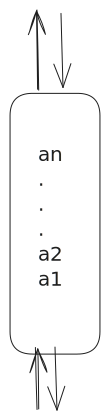
\includegraphics[width=0.1\textwidth]{./figure/pdf/cropped/DQueue.pdf}
  \caption{双端队列}
  \label{fig:deque}
\end{figure}


\section{栈和队列的应用}

\subsection{栈的应用}

\subsubsection{简单表达式求值}

这里限定的简单表达式是用户输入的一个包含+、-、*、/、(、)和正整数的合法算数表达式,计算该表达式的运算结果。

在算术表达式中, 运算符位于两个操作数中间的表达式称为中缀表达式 (infix
expression) ,例如 1十2* 3 就是一个中绥表达式。中组表达式是一种最常用的表达式形式,
日常生活中的表达式一般都是中绥表达式。

对中组表达式的运算一般遵循“先乘除,后加减,从左到右计算,先括号内,后括号外?的
规则,因此中组表达式不仅要依赖运算符优先级,还要处理括号。

算术表达式的另一种形式是后缀表达式(postfix expression)或逆波兰表达式,就是在
算术表达式中运算符在操作数的后面,如1+2* 3 的后组表达式为12 3 * +。在后缀表
达式中已经考虑了运算符的优先级,没有括号,只有操作数和运算符,而且越放在前面的运
算符越优先执行。

同样,在算术表达式中,如果运算符在操作数的前面,称为前缀表达式 (prefix
expression) ,如 1+2* 3 的前缀表达式为+1 * 2 3。

后缀表达式是一种十分有用的表达式,它将复杂表达式转换为可以依靠简单的操作得
到计算结果的表达式。所以对中绥表达式的求值过程是先将中绥算术表达式转换成后缀表
达式,然后对该后缀表达式求值。


\textbf{中缀表达式转后缀表达式}

中缀表达式转后缀表达式的算法如下:

1. 从左到右扫描中缀表达式。

2. 如果是操作数,则直接输出。

3. 如果是运算符,则判断其与栈顶运算符的优先级,是右括号或优先级低于栈顶运算符,则栈顶运算符依次出栈并输出,直到遇到左括号或栈空为止。此时将当前运算符入栈。

4. 如果是左括号,则直接入栈。

5. 如果是右括号,则依次出栈并输出直到遇到左括号,左括号出栈。

6. 重复2-5步骤,直到表达式的最右端。

7. 将栈中的运算符依次出栈并输出。

例如,中缀表达式$3+5*8-(6 + 2)$转换为后缀表达式的过程如表\ref{tab:infixToPostfix}所示。


\begin{table}[h!]
  \centering
  \begin{tabular}{|c|c|c|}
  \hline
  \textbf{扫描的符号} & \textbf{栈 (Stack)} & \textbf{输出 (Output)} \\ \hline
  3 &  & 3 \\ \hline
  + & + & 3 \\ \hline
  5 & + & 3 5 \\ \hline
  * & + * & 3 5 \\ \hline
  8 & + * & 3 5 8 \\ \hline
  - & - & 3 5 8 * + \\ \hline
  ( & - ( & 3 5 8 * + \\ \hline
  6 & - ( & 3 5 8 * + 6 \\ \hline
  + & - ( + & 3 5 8 * + 6 \\ \hline
  2 & - ( + & 3 5 8 * + 6 2 \\ \hline
  ) & - & 3 5 8 * + 6 2 + \\ \hline
  (结束) &  & 3 5 8 * + 6 2 + - \\ \hline
  \end{tabular}
  \caption{前缀转后缀}
  \label{tab:infixToPostfix}
  \end{table}

代码如代码\ref{lst:infixToPostfix}所示。

\begin{lstlisting}[language=C++, caption={中缀表达式转后缀表达式示例代码}, label={lst:infixToPostfix}]
  bool isOperator(char c) {
    return c == '+' || c == '-' || c == '*' || c == '/';
  }

  int priority(char c) {
    if (c == '+' || c == '-') {
      return 1;
    }
    if (c == '*' || c == '/') {
      return 2;
    }
    return 0;
  }

  string infixToPostfix(string infix) {
    stack<char> s;
    string postfix = "";
    for (int i = 0; i < infix.size(); i++) {
      if (isdigit(infix[i])) {
        postfix += infix[i];
      } else if (infix[i] == '(') {
        s.push(infix[i]);
      } else if (infix[i] == ')') {
        while (!s.empty() && s.top() != '(') {
          postfix += s.top();
          s.pop();
        }
        s.pop();
      } else if (isOperator(infix[i])) {
        while (!s.empty() && priority(s.top()) >= priority(infix[i])) {
          postfix += s.top();
          s.pop();
        }
        s.push(infix[i]);
      }
    }
    while (!s.empty()) {
      postfix += s.top();
      s.pop();
    }
    return postfix;
  }

\end{lstlisting}

该算法的总时间复杂度为 $O(n)$,空间复杂度为 $O(n)$。

特点:中缀表达式转后缀表达式。

\textbf{后缀表达式求值}

后缀表达式求值的算法如下:

1. 从左到右扫描后缀表达式。

2. 如果是操作数,则入栈。

3. 如果是运算符,则从栈中弹出两个操作数,进行运算,将运算结果入栈。

4. 重复2-3步骤,直到表达式的最右端。

5. 栈中的元素即为表达式的运算结果。

例如,后缀表达式$3 5 8 * + 6 2 + -$的求值过程如表\ref{tab:postfixEvaluation}所示。

\begin{table}[h!]
  \centering
  \begin{tabular}{|c|c|}
  \hline
  \textbf{扫描的符号} & \textbf{栈 (Stack)} \\ \hline
  3 & 3 \\ \hline
  5 & 3 5 \\ \hline
  8 & 3 5 8 \\ \hline
  * & 3 40 \\ \hline
  + & 43 \\ \hline
  6 & 43 6 \\ \hline
  2 & 43 6 2 \\ \hline
  + & 43 8 \\ \hline
  - & 35 \\ \hline
  \end{tabular}
  \caption{后缀表达式求值}
  \label{tab:postfixEvaluation}
  \end{table}

代码如代码\ref{lst:postfixEvaluation}所示。

\begin{lstlisting}[language=C++, caption={后缀表达式求值示例代码}, label={lst:postfixEvaluation}]
  int postfixEvaluation(string postfix) {
    stack<int> s;
    for (int i = 0; i < postfix.size(); i++) {
      if (isdigit(postfix[i])) {
        s.push(postfix[i] - '0');
      } else {
        int b = s.top();
        s.pop();
        int a = s.top();
        s.pop();
        if (postfix[i] == '+') {
          s.push(a + b);
        } else if (postfix[i] == '-') {
          s.push(a - b);
        } else if (postfix[i] == '*') {
          s.push(a * b);
        } else if (postfix[i] == '/') {
          s.push(a / b);
        }
      }
    }
    return s.top();
  }

\end{lstlisting}


\subsubsection{括号匹配}

括号匹配是指对于一个字符串,其中包含的括号必须是成对出现的,且左括号必须在右括号的前面。

例如,字符串“((()))”是括号匹配的,而字符串“(()))”不是括号匹配的。

括号匹配的算法如下:

1. 从左到右扫描字符串。

2. 如果是左括号,则入栈。

3. 如果是右括号,则判断栈是否为空,如果为空,则返回false;否则,出栈。

4. 重复2-3步骤,直到字符串的最右端。

5. 如果栈为空,则返回true;否则,返回false。

例如,字符串“(())()”的括号匹配过程如表\ref{tab:bracketMatching}所示。

\begin{table}[h!]
  \centering
  \begin{tabular}{|c|c|c|}
  \hline
  \textbf{扫描的符号} & \textbf{栈 (Stack)} & \textbf{是否匹配} \\ \hline
  ( & ( &  \\ \hline
  ( & (( &  \\ \hline
  ) & ( &  \\ \hline
  ) &  &  \\ \hline
  ( & ( &  \\ \hline
  ) &  &  \\ \hline
  (结束) &  & 是 \\ \hline
  \end{tabular}
  \caption{括号匹配}
  \label{tab:bracketMatching}
  \end{table}

代码如代码\ref{lst:bracketMatching}所示。

\begin{lstlisting}[language=C++, caption={括号匹配示例代码}, label={lst:bracketMatching}]
  bool bracketMatching(string s) {
    stack<char> st;
    for (int i = 0; i < s.size(); i++) {
      if (s[i] == '(') {
        st.push(s[i]);
      } else if (s[i] == ')') {
        if (st.empty()) {
          return false;
        }
        st.pop();
      }
    }
    return st.empty();
  }

\end{lstlisting}

该算法的总时间复杂度为 $O(n)$,空间复杂度为 $O(n)$。

特点:括号匹配。

\subsection{队列的应用}

\subsubsection{约瑟夫环问题}

约瑟夫环问题是一个著名的问题,是一个数学的应用问题,该问题的大致描述如下:

设有n个人围成一圈,从第一个人开始报数,报到m的人出列,然后从出列的下一个人开始重新报数,报到m的人出列,如此循环,直到所有的人都出列为止。

例如,当n=6,m=5时,出列的顺序为5、4、6、2、3、1。

约瑟夫环问题的算法如下:

1. 创建一个队列,将所有的人依次入队。

2. 从队头开始,依次出队,报数,如果报数为m,则出队;否则,重新入队。

3. 重复2步骤,直到队列为空。

例如,当n=6,m=5时,出列的顺序为5、4、6、2、3、1。

代码如代码\ref{lst:josephus}所示。

\begin{lstlisting}[language=C++, caption={约瑟夫环问题示例代码}, label={lst:josephus}]
  void josephus(int n, int m) {
    queue<int> q;
    for (int i = 1; i <= n; i++) {
      q.push(i);
    }
    while (!q.empty()) {
      for (int i = 1; i < m; i++) {
        q.push(q.front());
        q.pop();
      }
      cout << q.front() << " ";
      q.pop();
    }
  }

\end{lstlisting}

该算法的总时间复杂度为 $O(nm)$,空间复杂度为 $O(n)$。

特点:约瑟夫环问题。




\chapter{串}

串(string)是由零个或多个字符组成的有限序列。含零个字符的串称为空串,用多表
示。串中所含字符的个数称为该串的长度(或串长)。通常将一个串表示成"aa …a, 的形
式,其中最外边的双引号(或单引号)不是串的内容,它们是串的标志,用于将串与标识符(如
变量名等)加以区别。每个 w(1委未站代表一个字符,不同的机器和编程语言对合法字符
〈即人允许使用的字符)有不同的规定。但在一般情况下,英文字母.数字(0,1,…,9)和常用的
标点符号以及空格符等都是合法的字符。

两个串相等当且仅当这两个串的长度相等并且各对应位置上的字符都
相同。一个串中任意个连续字符组成的序列称为该串的子串(substring),
例如串"abcde"的子串有"a"、ab"、abc"和"abcd"等。为了表述清楚,在串
中空格字符用“0D"”符号表示,例如"aDOb"是一个长度为4的串,其中含有两
个空格字符。空串是不包含任何字符的串,其长度为 0,空串是任何串的
子串


\section{串的存储结构}

串的存储结构有两种,即顺序存储结构和链式存储结构。
\subsection{顺序存储结构}


顺序串中的字符被依次存放在一组连续的存储单元里。一般来说,一个字节(8 位)可
以表示一个字符(存放其 ASCII 码) 。而计算机内存是按字编址的,即以字为存储单位,一
个存储单元指的是一个字。而一个字可能包含多个字节,其所包含的字节数随机器而异。

顺序串的存储方式有两种: 一种是每个字只存一个字符,如图 4. 1 所示(假设一个字包
含4个字节) ,这称为非紧缩格式(其存储密度小); 另一种是每个字存放多个字符,如图 4. 2
所示 ,这称为紧缩格式(其存储密度大) 。在这两个图中,有阴影的字节为空闲部分。

非紧缩格式如表 \ref{}
\subsection{链式存储结构}

\section{串的操作}

\subsection{串的基本操作}

\subsection{模式匹配算法}

\subsubsection{BF算法}

\subsubsection{KMP算法}

\chapter{稀疏矩阵和广义表}

\section{稀疏矩阵}

\subsection{稀疏矩阵的定义}

\subsection{稀疏矩阵的三元组表示}

\section{广义表}

\subsection{广义表的定义}

\subsection{广义表的存储结构}

\subsection{广义表的运算}

\chapter{树}

\section{树的基本概念}

\subsection{树的定义}

\subsection{树的基本术语}

\subsection{树的基本性质}

\section{树的存储结构}

\subsection{顺序存储结构}

\subsection{链式存储结构}

\section{二叉树}

\subsection{二叉树的定义}

\subsection{二叉树的性质}

\subsection{二叉树的五种基本形态}

\subsection{特殊二叉树}

\subsubsection{满二叉树}

\subsubsection{完全二叉树}

\subsubsection{二叉搜索树}

\subsubsection{平衡二叉树}

\subsubsection{线索二叉树}

\section{二叉树的存储结构}

\subsection{顺序存储结构}

\subsection{链式存储结构}

\section{二叉树的遍历}

\subsection{遍历的定义}

\subsection{遍历的方法}

\subsubsection{递归遍历}

\paragraph{先序遍历}

\paragraph{中序遍历}

\paragraph{后序遍历}

\subsubsection{非递归遍历}

\paragraph{先序遍历}

\paragraph{中序遍历}

\paragraph{后序遍历}

\subsubsection{层次遍历}

\section{二叉树的基本运算}

\subsection{二叉树的创建}

\section{树、森林和二叉树的转换}

\subsection{树和森林的转换}

\subsection{二叉树和森林的转换}

\subsection{哈夫曼树和哈夫曼编码}

\subsection{并查集}

\chapter{图}

\section{图的基本概念}

\subsection{图的定义}

\subsection{图的分类}

\subsection{图的基本术语}

\section{图的存储结构}

\subsection{邻接矩阵}

\subsection{邻接表}

\subsection{十字链表}

\subsection{邻接多重表}

\section{图的遍历}

\subsection{深度优先搜索}

\subsection{广度优先搜索}

\section{最小生成树}

\subsection{Prim算法}

\subsection{Kruskal算法}

\section{最短路径}

\subsection{Dijkstra算法}

\subsection{Floyd算法}

\section{拓扑排序}

\section{关键路径}

\chapter{查找}

\section{查找的基本概念}

\subsection{查找的定义}

\subsection{查找的基本术语}

\section{顺序查找}

\section{折半查找}

\section{分块查找}

\section{哈希查找}

\section{红黑树}

\section{B树}

\section{B+树}

\chapter{排序}

\section{排序的基本概念}

\subsection{排序的定义}

\subsection{排序的基本术语}

\section{插入排序}

\subsection{直接插入排序}

\subsection{希尔排序}

\section{交换排序}

\subsection{冒泡排序}

\subsection{快速排序}

\section{选择排序}

\subsection{直接选择排序}

\subsection{堆排序}

\section{归并排序}

\section{基数排序}

\section{排序算法的比较}

\section{外部排序}

\end{document}
